\documentclass[11pt, reqno]{amsart}
\usepackage{amsfonts, amssymb, amscd, amsrefs}
\usepackage{graphicx}
\usepackage{hyperref}
\usepackage{slashed}
\usepackage{fullpage}

\begin{document}

\author{Giacinto Paolo Saggese}
\author{Paul Smith}

\thanks{With contributions from
	Samarth KaPatel,
	Grisha Pomazkin,
	Juraj Smeriga,
	Danya Tikhomirov,
	Nina Trubacheva,
	Dan Yachmenev,
	Vladimir Yakovenko,
	and
	Tamara Zhordaniya}

\date{\today}

\maketitle

% ###############################################################################
\section{Abstract}

Surrentum\footnote{Surrentum is the Latin name of the coastal city of
  Sorrento in the South of Italy. In Greek mythology it was the place
  inhabited by Sirens, who tried to seduce Ulysses in one of the
  episodes of the Odyssey.} is a protocol to:

\begin{itemize}
\item
  \begin{quote}
  implement distributed investment strategies
  \end{quote}
\item
  \begin{quote}
  enforce a unified view of market exchanges, both centralized and
  decentralized, with benefits to the efficiency of the entire system
  \end{quote}
\item
  \begin{quote}
  incentivize participants that stake their cryptocurrencies to provide
  liquidity to digital asset markets
  \end{quote}
\end{itemize}

Surrentum protocol contains:

\begin{itemize}
\item
  \begin{quote}
  A framework for describing, simulating, assessing, and deploying
  financial machine learning models operating on any object on a
  blockchain (e.g., cryptocurrencies, tokens, NFTs, smart contracts)
  \end{quote}
\item
  \begin{quote}
  A suite of standards for interoperability between components of the
  ecosystem (e.g., Surrentum Oracles, Surrentum Nodes, Market exchanges)
  \end{quote}
\item
  \begin{quote}
  Smart contracts allowing peer-to-peer staking of cryptocurrencies used
  to provide liquidity to the financial system and be rewarded with
  investment returns
  \end{quote}
\end{itemize}

% ###############################################################################
\section{Motivation}

Increasing adoption and continued decentralization of digital asset
markets fragments and distorts prices, leading to volatile markets.

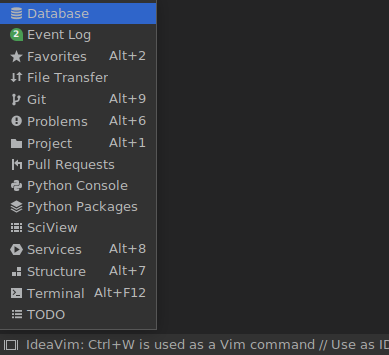
\includegraphics[width=6.5in,height=2.54167in]{media/image4.png}

At the current market capitalization of over \$2+ trillion and daily
trading volume exceeding \$50 billion across 20,000 currencies and 500
crypto exchanges, research estimates pricing inefficiencies in digital
markets to be between \$50m-200m per day.

The intrinsic appeals of crypto currency (i.e., the lack of a
centralized authority) and its rapid adoption across retail transactions
will only exacerbate the problem.

Historical solutions (e.g., Nasdaq regulation in the 1990s and US
Government Reg-NMS in 2005) have relied on government initiatives to
regulate stock exchanges and brokers to execute trades at the best
possible price across multiple exchanges. In the case of
cryptocurrencies, such a solution is impossible, given the decentralized
nature of its market and the ways in which consensus is achieved.

% ###############################################################################
\section{Asset representation}

TODO(gp): Ideally we want to use a single schema like
`Vendor:ExchangeId:Asset`

\textbackslash\# Asset universe

% ###############################################################################
\section{Surrentum Data Specification}

\subsection{ETL}

We employ a variation of the ETL approach, called EtLT (i.e., extract,
lightly transform, load, transform) for downloading both data and
metadata. We can have a different pipeline for data and one metadata.

Data is extracted from an external data source, lightly transformed, and
then loaded into permanent storage. Then downstream data pipelines read
the data with a standard client interface.

\textbf{Large variety of data.} Data comes in a very large variety, for
instance:

\begin{itemize}
\item
  \begin{quote}
  Different vendor can provide the same data
  \end{quote}

  \begin{itemize}
  \item
    \begin{quote}
    E.g., Kibot, Binance, CryptoDataDownload provide data for the
    Binance exchange
    \end{quote}
  \end{itemize}
\item
  \begin{quote}
  Different time semantics, e.g.,
  \end{quote}

  \begin{itemize}
  \item
    \begin{quote}
    Intervals can be {[}a, b) or (a, b{]}
    \end{quote}
  \item
    \begin{quote}
    A bar can be marked at the end or at the beginning of the interval
    \end{quote}
  \end{itemize}
\item
  \begin{quote}
  Data and metadata
  \end{quote}

  \begin{itemize}
  \item
    \begin{quote}
    Some vendors provide metadata, others don\textquotesingle t
    \end{quote}
  \end{itemize}
\item
  \begin{quote}
  Multiple asset classes (e.g., equities, futures, crypto)
  \end{quote}
\item
  \begin{quote}
  Data at different time resolutions, e.g.,
  \end{quote}

  \begin{itemize}
  \item
    \begin{quote}
    daily bars
    \end{quote}
  \item
    \begin{quote}
    minute bars
    \end{quote}
  \item
    \begin{quote}
    trades
    \end{quote}
  \item
    \begin{quote}
    order book data
    \end{quote}
  \end{itemize}
\item
  \begin{quote}
  Historical vs real-time
  \end{quote}
\item
  \begin{quote}
  Price data vs alternative data
  \end{quote}
\end{itemize}

\textbf{Storage backend}. Data can be saved in multiple storage
backends:

\begin{itemize}
\item
  \begin{quote}
  database (e.g., Postgres, MongoDB)
  \end{quote}
\item
  \begin{quote}
  local filesystem
  \end{quote}
\item
  \begin{quote}
  remote filesystems (e.g., AWS S3 bucket)
  \end{quote}
\end{itemize}

Data can be saved on filesystems in different formats (e.g., CSV, JSON,
Parquet).

\textbf{S3 vs local filesystem.} Unfortunately it's not easy to abstract
the differences between AWS S3 buckets and local filesystems, since the
S3 interface is more along a key-value store rather than a filesystem
(supporting permissions, deleting recursively a directory, moving,
etc.).

Solutions based on abstracting a filesystem on top of S3 (e.g., mounting
S3 with Fuse filesystems) are not robust enough.

Some backends (e.g., Parquet) allow handling an S3 bucket transparently.

Our typical approach is:

\begin{itemize}
\item
  \begin{quote}
  When writing to S3, use the local filesystem for staging the data in
  the desired structure and then copy all the data to S3
  \end{quote}
\item
  \begin{quote}
  When reading from S3, read the data directly, use the functionalities
  supported by the backend, or copy the data locally and then read it
  from local disk
  \end{quote}
\end{itemize}

\textbf{Data formats}. The main data formats that Surrentum supports
are:

\begin{itemize}
\item
  \begin{quote}
  CSV
  \end{quote}
\end{itemize}

\begin{itemize}
\item
  \begin{quote}
  Pros
  \end{quote}
\end{itemize}

\begin{itemize}
\item
  \begin{quote}
  Easy to inspect
  \end{quote}
\end{itemize}

\begin{itemize}
\item
  \begin{quote}
  Easy to load / save
  \end{quote}
\item
  \begin{quote}
  Everybody understands it
  \end{quote}
\end{itemize}

\begin{itemize}
\item
  \begin{quote}
  Cons
  \end{quote}

  \begin{itemize}
  \item
    \begin{quote}
    Data can\textquotesingle t be easily sliced by asset ids / by time
    \end{quote}
  \item
    \begin{quote}
    Large footprint (non binary), although it can be compressed (e.g.,
    as `.csv.gz` on the fly)
    \end{quote}
  \end{itemize}
\end{itemize}

\begin{itemize}
\item
  \begin{quote}
  Parquet
  \end{quote}
\end{itemize}

\begin{itemize}
\item
  \begin{quote}
  Pros
  \end{quote}

  \begin{itemize}
  \item
    \begin{quote}
    Compressed
    \end{quote}
  \item
    \begin{quote}
    AWS friendly
    \end{quote}
  \item
    \begin{quote}
    Data can be easily sliced by asset ids and time
    \end{quote}
  \end{itemize}
\item
  \begin{quote}
  Cons
  \end{quote}

  \begin{itemize}
  \item
    \begin{quote}
    Not easy to inspect
    \end{quote}

    \begin{itemize}
    \item
      \begin{quote}
      Solution: use wrapper to convert to CSV
      \end{quote}
    \end{itemize}
  \item
    \begin{quote}
    Difficult to append
    \end{quote}

    \begin{itemize}
    \item
      \begin{quote}
      Solution: use chunking + defragmentation
      \end{quote}
    \end{itemize}
  \item
    \begin{quote}
    Cumbersome for real-time data
    \end{quote}
  \end{itemize}
\end{itemize}

\begin{itemize}
\item
  \begin{quote}
  database
  \end{quote}
\end{itemize}

\begin{itemize}
\item
  \begin{quote}
  Pros
  \end{quote}

  \begin{itemize}
  \item
    \begin{quote}
    Easy to inspect
    \end{quote}
  \item
    \begin{quote}
    Support any access pattern
    \end{quote}
  \item
    \begin{quote}
    Friendly for real-time data
    \end{quote}
  \end{itemize}
\item
  \begin{quote}
  Cons
  \end{quote}

  \begin{itemize}
  \item
    \begin{quote}
    Need devops to manage database instance
    \end{quote}
  \item
    \begin{quote}
    Difficult to track lineage and version
    \end{quote}
  \end{itemize}
\end{itemize}

Unfortunately there is not an obvious best solution so we have to deal
with multiple representations and transforming between them. In practice
Parquet is better suited to store historical data and database to store
real time data.

\textbf{Extract stage}. The goal is to acquire raw data from an external
source and archive it into a permanent storage backend (e.g.,
file-system and/or database). The data can be either historical or
real-time. We typically don\textquotesingle t process the data at all,
but rather we prefer to save the data raw as it comes from the wire.

\textbf{Transform stage}. Typically we prefer to load the data in the
backend with minor or no transformation. Specifically we allow changing
the representation of the data / format (e.g., removing some totally
useless redundancy, compressing the data, transforming from strings to
datetimes). We don't allow changing the semantics or filter columns.
This is done dynamically in the `client` stage

\textbf{Load stage.} The load stage simply saves the data into one of
the supported backends.

Typically we prefer to save

\begin{itemize}
\item
  \begin{quote}
  Historical data into Parquet format since it supports more naturally
  the access patterns needed for long simulations
  \end{quote}
\item
  \begin{quote}
  Real-time data into a database since this makes it easy to append and
  retrieve data in real-time. Often we want to also append real-time
  data to Parquet
  \end{quote}
\end{itemize}

Client stage. The client stage allows downstream pipelines to access
data from the backend storage. The access pattern is always for a model
is always "give me the columns XYZ for assets ABC in the period {[}...,
...{]}".

We prefer to perform some transformations that are lightweight (e.g.,
converting Unix epochs in timestamps) or still evolving (e.g.,
understanding the timing semantic of the data) are performed inside this
stage, rather than in the transform stage.

\textbf{ETL primitives}. We implement basic primitives that can be
combined in different ways to create various ETL pipelines.

\begin{itemize}
\item
  \begin{quote}
  Extract:
  \end{quote}

  \begin{itemize}
  \item
    \begin{quote}
    Read data from an external source to memory (typically in the form
    of Pandas data structures)
    \end{quote}
  \item
    \begin{quote}
    E.g., downloading data from a REST or Websocket interface
    \end{quote}
  \end{itemize}
\end{itemize}

\begin{itemize}
\item
  \begin{quote}
  Load:
  \end{quote}

  \begin{itemize}
  \item
    \begin{quote}
    Load data stored in memory -\textgreater{} permanent storage (e.g.,
    save as CSV or as Parquet)
    \end{quote}
  \item
    \begin{quote}
    E.g., pd.to\_parquet()
    \end{quote}
  \item
    \begin{quote}
    DbSave
    \end{quote}

    \begin{itemize}
    \item
      \begin{quote}
      Save to DB
      \end{quote}
    \item
      \begin{quote}
      Create schema
      \end{quote}
    \end{itemize}
  \end{itemize}
\end{itemize}

\begin{itemize}
\item
  \begin{quote}
  Client:
  \end{quote}

  \begin{itemize}
  \item
    \begin{quote}
    From a permanent storage (e.g., disk) -\textgreater{} Memory
    \end{quote}
  \item
    \begin{quote}
    E.g., pd.from\_parquet()
    \end{quote}
  \end{itemize}
\end{itemize}

\begin{itemize}
\item
  \begin{quote}
  ClientFromDb
  \end{quote}

  \begin{itemize}
  \item
    \begin{quote}
    DB -\textgreater{} Memory
    \end{quote}
  \item
    \begin{quote}
    Creates the SQL query to read the data
    \end{quote}
  \end{itemize}
\end{itemize}

\begin{itemize}
\item
  \begin{quote}
  Validator
  \end{quote}

  \begin{itemize}
  \item
    \begin{quote}
    https://github.com/cryptokaizen/cmamp/pull/3386/files
    \end{quote}
  \end{itemize}
\end{itemize}

\begin{itemize}
\item
  \begin{quote}
  Transform
  \end{quote}
\end{itemize}

\begin{itemize}
\item
  \begin{quote}
  Just a class
  \end{quote}
\end{itemize}

\textbf{Example of ETL pipelines.}

\begin{itemize}
\item
  \begin{quote}
  Download historical data and save it as CSV or PQ
  \end{quote}
\item
  \begin{quote}
  Download order book data, compress it, and save it on S3
  \end{quote}
\item
  \begin{quote}
  Insert 1 minute worth of data in the DB
  \end{quote}

  \begin{itemize}
  \item
    \begin{quote}
    Write data into DB
    \end{quote}

    \begin{itemize}
    \item
      \begin{quote}
      One could argue that operations on the DB might not look like
      `extract` but rather `load`
      \end{quote}
    \item
      \begin{quote}
      We treat any backend (S3, local, DB) in the same way and the DB is
      just a backend
      \end{quote}
    \end{itemize}
  \end{itemize}
\item
  \begin{quote}
  \href{https://docs.google.com/document/d/1EH7RqeTdVCXDcrCKPm0PvrtftTA11X9V-AT7F20V7T4/edit\#heading=h.t1ycoe6irr95}{\ul{More
  detailed description}}
  \end{quote}

  \begin{itemize}
  \item
    \begin{quote}
    \textbf{Examples}:
    \end{quote}

    \begin{itemize}
    \item
      \begin{quote}
      Transformations CSV -\textgreater{} Parquet
      \textless-\textgreater{} DB
      \end{quote}
    \item
      \begin{quote}
      Convert the CSV data into Parquet using certain indices
      \end{quote}
    \item
      \begin{quote}
      Convert Parquet by-date into Parquet by-asset
      \end{quote}
    \end{itemize}
  \end{itemize}
\end{itemize}

% ===============================================================================
\subsection{Data pipelines}

Download data by asset (as a time series)

\begin{itemize}
\item
  \begin{quote}
  asset.csv.gz or Parquet
  \end{quote}
\item
  \begin{quote}
  Historical format
  \end{quote}
\end{itemize}

Download data by time, e.g.,

\begin{itemize}
\item
  \begin{quote}
  20211105/\ldots{}
  \end{quote}
\item
  \begin{quote}
  csv.gz or Parquet
  \end{quote}
\item
  \begin{quote}
  This is typical of real-time flow
  \end{quote}
\end{itemize}

% ===============================================================================
\subsection{General conventions}

\textbf{Data invariants}. We use the following invariants when storing
data during data on-boarding and processing:

\begin{itemize}
\item
  \begin{quote}
  Data quantities are associated to intervals are {[}a, b) (e.g., the
  return over an interval) or to a single point in time (e.g., the close
  price at 9am UTC)
  \end{quote}
\item
  \begin{quote}
  Every piece of data is labeled with the end of the sampling interval
  or with the point-in-time
  \end{quote}

  \begin{itemize}
  \item
    \begin{quote}
    E.g., for a quantity computed in an interval {[}06:40:00, 06:41:00)
    the timestamp is 06:41:00
    \end{quote}
  \end{itemize}
\item
  \begin{quote}
  Timestamps are always time-zone aware and use UTC timezone
  \end{quote}
\item
  \begin{quote}
  Every piece of data has a knowledge timestamp (aka "as-of-date") which
  represent when we were aware of the data according to our wall-clock:
  \end{quote}

  \begin{itemize}
  \item
    \begin{quote}
    Multiple timestamps associated with different events can be tracked,
    e.g., `start\_download\_timestamp`, `end\_download\_timestamp`
    \end{quote}
  \item
    \begin{quote}
    No system should depend on data available strictly before the
    knowledge timestamp
    \end{quote}
  \end{itemize}
\item
  \begin{quote}
  Data is versioned: every time we modify the schema or the semantics of
  the data, we bump up the version using semantic versioning and update
  the changelog of what each version contains
  \end{quote}
\end{itemize}

An example of tabular data is below:

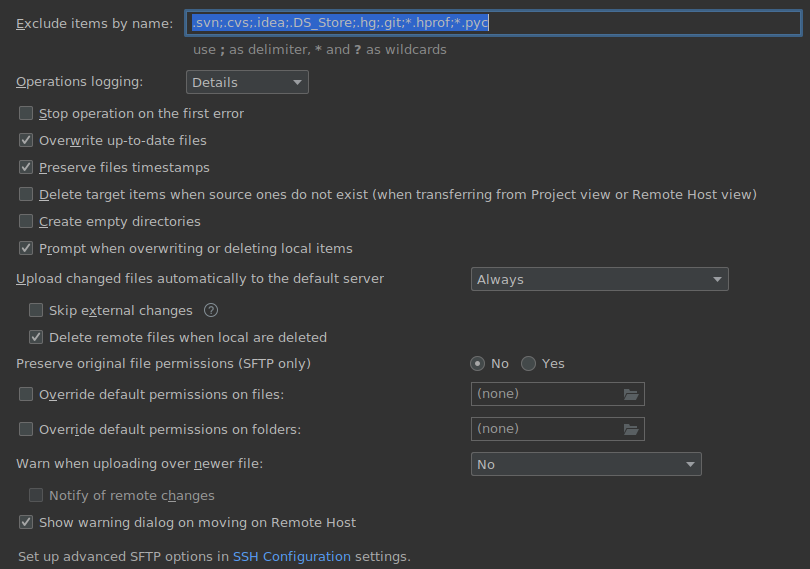
\includegraphics[width=6.5in,height=1.01389in]{media/image2.png}

\textbf{Data organization}. We keep data together by execution run
instead of by data element.

E.g., assume we run a flow called `XYZ\_sanity\_check` every day and the
flow generates three pieces of data, one file `output.txt` and two
directories `logs`, `temp\_data`.

We want to organize the data in a directory structure like:

\emph{\textbf{Better}}

```

\begin{itemize}
\item
  \begin{quote}
  XYZ\_sanity\_check/
  \end{quote}

  \begin{itemize}
  \item
    \begin{quote}
    run.\{date\}/
    \end{quote}

    \begin{itemize}
    \item
      \begin{quote}
      output.txt
      \end{quote}
    \item
      \begin{quote}
      logs/
      \end{quote}
    \item
      \begin{quote}
      temp\_data/
      \end{quote}
    \end{itemize}
  \item
    \begin{quote}
    run.\{date\}.manual/
    \end{quote}

    \begin{itemize}
    \item
      \begin{quote}
      output.txt
      \end{quote}
    \item
      \begin{quote}
      logs/
      \end{quote}
    \item
      \begin{quote}
      temp\_data/
      \end{quote}
    \end{itemize}
  \end{itemize}
\end{itemize}

```

\emph{\textbf{Worse}}

```

\begin{itemize}
\item
  \begin{quote}
  XYZ\_sanity\_check/
  \end{quote}

  \begin{itemize}
  \item
    \begin{quote}
    output.\{date\}/
    \end{quote}

    \begin{itemize}
    \item
      \begin{quote}
      output.txt
      \end{quote}
    \end{itemize}
  \item
    \begin{quote}
    logs.\{date\}/
    \end{quote}
  \item
    \begin{quote}
    temp\_data.\{date\}/
    \end{quote}
  \end{itemize}
\end{itemize}

```

The reasons why the first data layout is superior are:

\begin{enumerate}
\def\labelenumi{\arabic{enumi})}
\item
  \begin{quote}
  It\textquotesingle s easier to delete a single run by deleting a
  single dir instead of deleting multiple files
  \end{quote}
\item
  \begin{quote}
  It allows the format of the data to evolve over time without having to
  change the schema of the data retroactively
  \end{quote}
\item
  \begin{quote}
  It allows scripts post-processing the data to point to a directory
  with a specific run and work out of the box
  \end{quote}
\item
  \begin{quote}
  it\textquotesingle s easier to move the data for a single run from one
  dir (e.g., locally) to another (e.g., a central location) in one
  command
  \end{quote}
\item
  \begin{quote}
  there is redundancy and visual noise, e.g., the same data is
  everywhere
  \end{quote}
\end{enumerate}

We can tag directory by a run mode (e.g., `manual` vs `scheduled`) by
adding the proper suffix to a date-dir.

\textbf{Directory with one file}. Having a directory containing one
single file often creates redundancy.

We prefer not to use directories unless they contain more than one file.
We can use directories if we believe that it\textquotesingle s highly
likely that more files will be needed, but as often happens YANGI (you
are not going to need it) applies.

\textbf{Naming convention}.

\begin{itemize}
\item
  \begin{quote}
  We use `.` to separate conceptually different pieces of a file or a
  directory.
  \end{quote}
\item
  \begin{quote}
  We don\textquotesingle t allow white spaces since they are not Linux
  friendly and need to be escaped. We replace white spaces with `\_`.
  \end{quote}
\item
  \begin{quote}
  We prefer not to use `-` whenever possible, since they create issues
  with Linux auto-completion and need to be escaped.
  \end{quote}
\end{itemize}

E.g., `bulk.airflow.csv` instead of `bulk\_airflow.csv`

\textbf{Data pipeline classification}. A data pipeline can be any of the
following:

\begin{itemize}
\item
  \begin{quote}
  a downloader
  \end{quote}

  \begin{itemize}
  \item
    \begin{quote}
    External DB (e.g., data provider) -\textgreater{} Internal DB: the
    data flows from an external API to an internal DB
    \end{quote}
  \item
    \begin{quote}
    It downloads historical or real-time data and saves the dataset in a
    location
    \end{quote}
  \item
    \begin{quote}
    The name of the script and the location of the data downloaded
    follow the naming scheme described below
    \end{quote}
  \item
    \begin{quote}
    It is typically implemented as a Python script
    \end{quote}
  \end{itemize}
\item
  \begin{quote}
  a QA flow for a single or multiple datasets
  \end{quote}

  \begin{itemize}
  \item
    \begin{quote}
    Internal DB -\textgreater{} Process
    \end{quote}
  \item
    \begin{quote}
    It computes some statistics from one or more datasets (primary or
    derived) and throws an exception if the data is malformed
    \end{quote}
  \item
    \begin{quote}
    It aborts if the data has data not compliant to certain QA metrics
    \end{quote}
  \item
    \begin{quote}
    It is typically implemented as a Python notebook backed by a Python
    library
    \end{quote}
  \end{itemize}
\item
  \begin{quote}
  a derived dataset flow
  \end{quote}

  \begin{itemize}
  \item
    \begin{quote}
    Internal DB -\textgreater{} Process -\textgreater{} Internal DB
    \end{quote}
  \item
    \begin{quote}
    It computes some data derived from an existing data set
    \end{quote}

    \begin{itemize}
    \item
      \begin{quote}
      E.g., resampling, computing features
      \end{quote}
    \end{itemize}
  \item
    \begin{quote}
    It is typically implemented as a Python script
    \end{quote}
  \end{itemize}
\item
  \begin{quote}
  a model flow
  \end{quote}

  \begin{itemize}
  \item
    \begin{quote}
    Internal DB -\textgreater{} Process -\textgreater{} Outside DB
    (e.g., exchange)
    \end{quote}
  \item
    \begin{quote}
    E.g., it runs a computation from internal data and places some
    trades
    \end{quote}
  \item
    \begin{quote}
    It is typically implemented as a Python script
    \end{quote}
  \end{itemize}
\end{itemize}

\textbf{Data classification}. Data can be from market sources or from
non-market (aka alternative) sources. Each data source can come with
metadata, e.g.,

\begin{itemize}
\item
  \begin{quote}
  List of assets in the universe over time
  \end{quote}
\item
  \begin{quote}
  Attributes of assets (e.g., industry and other classification)
  \end{quote}
\end{itemize}

\textbf{Asset universe}. Often the data relates to a set of assets,
e.g., currency pairs on different exchanges. The support of the data is
referred to as the "data universe". This metadata is versioned as any
other piece of data.

% ===============================================================================
\subsection{Data set downloading and handling}

\textbf{Data set naming scheme}. Each data set is stored in a data lake
with a path and name that describe its metadata according to the
following signature:

dataset\_signature=\{download\_mode\}.\{downloading\_entity\}.\{action\_tag\}.\{data\_format\}.\{data\_type\}.\{asset\_type\}.\{universe\}.\{vendor\}.\{exchange\_id\}.\{version{[}-snapshot{]}\}.\{extension\}

TODO(gp): @juraj add a \{backend\} = s3, postgres, mongo, local\_file

The signature schema might be dependent on the backend

E.g.,
bulk/airflow/downloaded\_1min/csv/ohlcv/futures/universe\_v1\_0/ccxt/binance/v1\_0-20220210/BTC\_USD.csv.gz

We use `-` to separate pieces of the same attribute (e.g., version and
snapshot) and `\_` as replacements of a space character.

The organization of files in directories should reflect the naming
scheme. We always use one directory per attribute for files (e.g.,
`bulk.airflow.csv/...` or `bulk/airflow/csv/...`). When the metadata is
used not to identify a file in the filesystem (e.g., for a script or as
a tag) then we use `.` as separators between the attributes.

\textbf{Data set attributes}. There are several "attributes" of a data
set:

\begin{itemize}
\item
  \begin{quote}
  `download\_mode`: the type of downloading mode
  \end{quote}
\end{itemize}

\begin{itemize}
\item
  \begin{quote}
  `bulk`
  \end{quote}

  \begin{itemize}
  \item
    \begin{quote}
    Aka "one-shot", "one-off", and improperly "historical"
    \end{quote}
  \item
    \begin{quote}
    Data downloaded in bulk mode, as one-off documented operations
    \end{quote}
  \item
    \begin{quote}
    Sometimes it\textquotesingle s referred to as "historical", since
    one downloads the historical data in bulk before the real-time flow
    is deployed
    \end{quote}
  \end{itemize}
\item
  \begin{quote}
  `periodic`
  \end{quote}

  \begin{itemize}
  \item
    \begin{quote}
    Aka "scheduled", "streaming", "continuous", and improperly
    "real-time"
    \end{quote}
  \item
    \begin{quote}
    Data is captured regularly and continuously
    \end{quote}
  \item
    \begin{quote}
    Sometimes it\textquotesingle s referred as to "real-time" since one
    capture this data
    \end{quote}
  \item
    \begin{quote}
    It can contain information about the frequency of downloading (e.g.,
    `periodic-5mins`, `periodic-EOD`) if it needs to be identified with
    respect to others
    \end{quote}
  \end{itemize}
\item
  \begin{quote}
  `unit\_test`
  \end{quote}

  \begin{itemize}
  \item
    \begin{quote}
    Data used for unit test (independently if it was downloaded
    automatically or created manually)
    \end{quote}
  \end{itemize}
\item
\end{itemize}

\begin{itemize}
\item
  \begin{quote}
  `downloading\_entity`: different data depending on whom downloaded it,
  e.g.,
  \end{quote}
\end{itemize}

\begin{itemize}
\item
  \begin{quote}
  `airflow`: data was downloaded as part of the automatic flow
  \end{quote}
\item
  \begin{quote}
  `manual`: data download was triggered manually (e.g., running the
  download script)
  \end{quote}
\end{itemize}

\begin{itemize}
\item
  \begin{quote}
  `action\_tag`: information about the downloading, e.g.,
  `downloaded\_1min` or `downloaded\_EOD`
  \end{quote}
\item
  \begin{quote}
  `data\_format`: the format of the data, e.g.,
  \end{quote}
\end{itemize}

\begin{itemize}
\item
  \begin{quote}
  `csv` (always csv.gz, there is no reason for not compressing the data)
  \end{quote}
\item
  \begin{quote}
  `parquet`
  \end{quote}
\end{itemize}

\begin{itemize}
\item
  \begin{quote}
  `data\_type`: what type of data is stored, e.g.,
  \end{quote}
\end{itemize}

\begin{itemize}
\item
  \begin{quote}
  `ohlcv`, `bid\_ask`, `market\_depth` (aka `order\_book`),
  `bid\_ask\_market\_data` (if it includes both), `trades`
  \end{quote}
\end{itemize}

\begin{itemize}
\item
  \begin{quote}
  `asset\_type`: what is the asset class
  \end{quote}
\end{itemize}

\begin{itemize}
\item
  \begin{quote}
  E.g., futures, spot, options
  \end{quote}
\end{itemize}

\begin{itemize}
\item
  \begin{quote}
  `universe`: the name of the universe containing the possible assets
  \end{quote}

  \begin{itemize}
  \item
    \begin{quote}
    Typically the universe can have further characteristics and it can
    be also versioned
    \end{quote}
  \item
    \begin{quote}
    E.g., `universe\_v1\_7`
    \end{quote}
  \end{itemize}
\item
  \begin{quote}
  `vendor`: the source that provided the data
  \end{quote}

  \begin{itemize}
  \item
    \begin{quote}
    Aka ``provider''
    \end{quote}
  \end{itemize}
\end{itemize}

\begin{itemize}
\item
  \begin{quote}
  E.g., `ccxt`, `crypto\_chassis`, `cryptodata\_download`, `talos`,
  `kaiko`,
  \end{quote}
\item
  \begin{quote}
  Data can also be downloaded directly from an exchange (e.g.,
  `coinbase`, `binance`)
  \end{quote}
\item
  \begin{quote}
  `exchange\_id`: which exchange the data refers to
  \end{quote}
\end{itemize}

\begin{itemize}
\item
  \begin{quote}
  E.g., `binance`
  \end{quote}
\end{itemize}

\begin{itemize}
\item
  \begin{quote}
  `version`: any data set needs to have a version
  \end{quote}

  \begin{itemize}
  \item
    \begin{quote}
    Version is represented as major, minor, patch according to semantic
    versioning in the format `v\{a\}\_\{b\}\_\{c\}` (e.g., v1\_0\_0)
    \end{quote}
  \item
    \begin{quote}
    If the schema of the data is changed the major version is increased
    \end{quote}
  \item
    \begin{quote}
    If a bug is fixed in the downloader that improves the semantic of
    the data but it\textquotesingle s not a backward incompatible
    change, the minor version is increased
    \end{quote}
  \item
    \begin{quote}
    The same version can also include an optional `snapshot` which
    refers to the date when the data was downloaded (e.g., a specific
    date `20220210` to represent when the day on which the historical
    data was downloaded, i.e., the data was the historical data as-of
    2022-02-10)
    \end{quote}
  \item
    \begin{quote}
    Note that `snapshot` and `version` have an overlapping but not
    identical meaning. `snapshot` represents when the data was
    downloaded, while `version` refers to the evolution of the semantic
    of the data and of the downloader. E.g., the same data source can be
    downloaded manually on different days with the same downloader (and
    thus with the same version).
    \end{quote}
  \end{itemize}
\end{itemize}

\begin{itemize}
\item
  \begin{quote}
  `asset\_type`: which cryptocurrency the data refers to:
  \end{quote}

  \begin{itemize}
  \item
    \begin{quote}
    Typically there is one file per asset (e.g., `BTC\_USDT.csv.gz`)
    \end{quote}
  \item
    \begin{quote}
    Certain data formats can organize the data in a more complex way
    \end{quote}

    \begin{itemize}
    \item
      \begin{quote}
      E.g., Parquet files save the data in a directory structure
      `\{asset\}/\{year\}/\{month\}/data.parquet`
      \end{quote}
    \end{itemize}
  \end{itemize}
\end{itemize}

It is possible that a single data set covers multiple values of a
specific attribute

\begin{itemize}
\item
  \begin{quote}
  E.g., a data set storing data for both futures and spot, can have
  `asset\_type=futures\_spot`
  \end{quote}
\end{itemize}

Not all the cross-products are possible, e.g.

\begin{itemize}
\item
  \begin{quote}
  there is no data set with `download\_mode=periodic` scheduled by
  Airflow and `downloading\_entity=manual`
  \end{quote}
\end{itemize}

We organize the schema in terms of access pattern for the modeling and
analysis stage

\begin{itemize}
\item
  \begin{quote}
  E.g., `snapshot` comes before `vendor` since in different snapshots we
  can have different universes
  \end{quote}
\item
  \begin{quote}
  E.g., snapshot -\textgreater{} dataset -\textgreater{} vendor
  -\textgreater{} exchange -\textgreater{} coin
  \end{quote}
\end{itemize}

\begin{itemize}
\item
  \begin{quote}
  A universe is just a mapping of a tag (e.g., v5) to a set of
  directories
  \end{quote}
\end{itemize}

Each data set has multiple columns.

\textbf{References}.

The list of data sources on CK S3 bucket is
\href{https://docs.google.com/document/d/1C-22QF_gOe1k4HgyD6E6iOO_F_FxKKECd4MXaJEuTxo/edit\#heading=h.azfdjheqqtp}{\ul{Bucket
data organization}}

Useful notebooks for processing data is
\href{https://docs.google.com/document/d/17N8OTI1zxXI-l3OYDVcft1spDf0-JPUU8UiNCfBLYvY/edit\#heading=h.uxyv8hg7offz}{\ul{Master
notebooks}}

CK data specs:
\href{https://docs.google.com/document/d/1nLhaFBSHVrexCcwJMnpXlkqwn0l6bDiVer34GKVclYY/edit\#}{\ul{Data
pipelines - Specs}}

% ===============================================================================
\subsection{Data on-boarding flow}

\textbf{Downloader types.} For each data set, there are typically two
types of downloaders: bulk and periodic. This step is often the
equivalent of the Extract phase in an ETL / ELT / EtLT pipeline.

E.g., an EtLT pipeline can consists of the following phases:

\begin{itemize}
\item
  \begin{quote}
  E: extract 1 minute data from websocket,
  \end{quote}
\item
  \begin{quote}
  t: apply non-business logic related transformation from JSON to
  dataframe
  \end{quote}
\item
  \begin{quote}
  L: load into SQL
  \end{quote}
\item
  \begin{quote}
  T: transform the data resampling to 5 minute data
  \end{quote}
\end{itemize}

\textbf{Bulk downloaders}. Download past data querying from an API.

A characteristic of bulk downloaders is that the download is not
scheduled to be repeated on a regular basis. It is mostly executed once
(e.g., to get the historical data) or a few times (e.g., to catch up
with an intermittent data feed). It is executed (or at least triggered)
manually.

The data is downloaded in bulk mode at \$T\_\{dl,bulkhist\}\$ to catch
up with the historical data up to the moment of the deployment of the
periodic downloader scheduled every period \$\textbackslash Delta
t\_\{deploy,periodic\}\$.

The bulk download flow is also needed any time we need to "catch up"
with a missing periodic download, e.g., if the real-time capture system
was down.

\textbf{Preferred bulk data format}. Typically the data is saved in a
format that allows data to be loaded depending on what\textquotesingle s
needed from downstream systems (e.g., Parquet using tiles on assets and
period of times).

\textbf{Periodic downloaders}. Download the data querying an API every
period \$\textbackslash Delta T\_\{dl,periodic\}\$, which depends on the
application needs, e.g., every second, minute. Typically periodic
downloaders are triggered automatically (e.g., by a workflow
orchestrator like Apache Airflow).

Another possible name is "streaming" data. Typical example is a
websocket feed of continuous data.

\textbf{Preferred real-time data format}. Typically we save data in a DB
to be able to easily query the data from the model. Often we also save
data to an historical-like format to have a backup copy of the data.
Parquet format is not ideal since it\textquotesingle s not easy to
append data.

TODO(gp): Add diagram

Providers -\textgreater{} us

It\textquotesingle s the extract in ETL

\textbf{Downloader naming scheme.} A downloader has a name that
represents the characteristics of the data that is being downloaded in
the format above.

The downloaders usually don't encapsulate logic to download only a
single dataset. This means that the naming conventions for downloaders
are less strict than for the datasets themselves.

\begin{itemize}
\item
  \begin{quote}
  More emphasis is put into providing a comprehensive docstring
  \end{quote}
\item
  \begin{quote}
  We can\textquotesingle t use `.` in filenames as attribute separators
  because Python uses them to separate packages in import statements, so
  we replace them with `\_` in scripts
  \end{quote}
\item
  \begin{quote}
  The name should capture the most general use-case
  \end{quote}

  \begin{itemize}
  \item
    \begin{quote}
    E.g. if a downloader can download both OHLCV and Bid/Ask data for
    given exchange in a given time interval and save to relational DB or
    S3 we can simply name it `download\_exchange\_data.py`
    \end{quote}
  \end{itemize}
\end{itemize}

TODO(Juraj): explain that Airflow DAG names follow similar naming
conventions

Notebooks and scripts follow the naming scheme using a description
(e.g., `resampler`, `notebook`) instead of `downloader` and a proper
suffix (e.g., ipynb, py, sh)

TODO(gp): The first cell of a notebook contains a description of the
content, including which checks are performed

Production notebooks decide what is an error, by asserting

\textbf{Idempotency and catch-up mode}. TODO(gp): Add a paragraph on
this.

This is used for any data pipeline (both downloading and processing).

\textbf{Example}. An example of system downloading price data has the
following components

\begin{longtable}[]{@{}
  >{\raggedright\arraybackslash}p{(\columnwidth - 10\tabcolsep) * \real{0.1106}}
  >{\raggedright\arraybackslash}p{(\columnwidth - 10\tabcolsep) * \real{0.2197}}
  >{\raggedright\arraybackslash}p{(\columnwidth - 10\tabcolsep) * \real{0.2213}}
  >{\raggedright\arraybackslash}p{(\columnwidth - 10\tabcolsep) * \real{0.1347}}
  >{\raggedright\arraybackslash}p{(\columnwidth - 10\tabcolsep) * \real{0.1892}}
  >{\raggedright\arraybackslash}p{(\columnwidth - 10\tabcolsep) * \real{0.1245}}@{}}
\toprule\noalign{}
\begin{minipage}[b]{\linewidth}\raggedright
\textbf{Action}
\end{minipage} & \begin{minipage}[b]{\linewidth}\raggedright
\textbf{Dataset signature}
\end{minipage} & \begin{minipage}[b]{\linewidth}\raggedright
\textbf{Frequency}
\end{minipage} & \begin{minipage}[b]{\linewidth}\raggedright
\textbf{Dashboard}
\end{minipage} & \begin{minipage}[b]{\linewidth}\raggedright
\textbf{Data location}
\end{minipage} & \begin{minipage}[b]{\linewidth}\raggedright
\textbf{Active?}
\end{minipage} \\
\begin{minipage}[b]{\linewidth}\raggedright
Historical download
\end{minipage} & \begin{minipage}[b]{\linewidth}\raggedright
\end{minipage} & \begin{minipage}[b]{\linewidth}\raggedright
\begin{itemize}
\item
  All of the past day data
\item
  Once a day at 0:00:00 UTC
\end{itemize}
\end{minipage} & \begin{minipage}[b]{\linewidth}\raggedright
https://
\end{minipage} & \begin{minipage}[b]{\linewidth}\raggedright
s3://...
\end{minipage} & \begin{minipage}[b]{\linewidth}\raggedright
Yes
\end{minipage} \\
\begin{minipage}[b]{\linewidth}\raggedright
Real-time download
\end{minipage} & \begin{minipage}[b]{\linewidth}\raggedright
\end{minipage} & \begin{minipage}[b]{\linewidth}\raggedright
\begin{itemize}
\item
  Last minute data
\item
  Every minute
\end{itemize}
\end{minipage} & \begin{minipage}[b]{\linewidth}\raggedright
...
\end{minipage} & \begin{minipage}[b]{\linewidth}\raggedright
s3://...
\end{minipage} & \begin{minipage}[b]{\linewidth}\raggedright
Yes
\end{minipage} \\
\midrule\noalign{}
\endhead
\bottomrule\noalign{}
\endlastfoot
\end{longtable}

\href{https://docs.google.com/document/d/14C4PFU1nNd0l7sBLCz5DxvrTk_nakmiTHwCVbIUwgfs/edit\#heading=h.ntti3mum3dph}{\ul{Airflow
Active}}
\href{https://docs.google.com/document/d/14C4PFU1nNd0l7sBLCz5DxvrTk_nakmiTHwCVbIUwgfs/edit\#heading=h.ntti3mum3dph}{\ul{Downloaders}}

Describe ETL layer from
\href{https://docs.google.com/document/d/1C-22QF_gOe1k4HgyD6E6iOO_F_FxKKECd4MXaJEuTxo/edit\#heading=h.iwaxiv19a4zu}{\ul{Design
- Software components}}

\href{https://docs.google.com/document/d/1nLhaFBSHVrexCcwJMnpXlkqwn0l6bDiVer34GKVclYY/edit}{\ul{OHLCV
data pipeline}}

% ===============================================================================
\subsection{Data QA workflows}

\textbf{Quality-assurance metrics}. Each data set has QA metrics
associated with it to make sure the data has the minimum expected data
quality.

\begin{itemize}
\item
  \begin{quote}
  E.g., for 1-minute OHLCV data, the possible QA metrics are:
  \end{quote}

  \begin{itemize}
  \item
    \begin{quote}
    missing bars (timestamp)
    \end{quote}
  \item
    \begin{quote}
    missing / nan OHLCV values within an individual bar
    \end{quote}
  \item
    \begin{quote}
    points with volume = 0
    \end{quote}
  \item
    \begin{quote}
    data points where OHLCV data is not in the correct relationship
    (e.g., H and L are not higher or lower than O and C),
    \end{quote}
  \item
    \begin{quote}
    data points where OHLCV data are outliers (e.g., they are more than
    N standard deviations from the running mean)
    \end{quote}
  \end{itemize}
\end{itemize}

\textbf{Bulk data single-dataset QA metrics}. It is possible to run the
QA flow to compute the quality of the historical data. This is done
typically as a one-off operation right after the historical data is
downloaded in bulk. This touches only one dataset, namely the one that
was just downloaded.

\begin{itemize}
\tightlist
\item
\end{itemize}

\textbf{Periodic QA metrics}. Every N minutes of downloading real-time
data, the QA flow is run to generate statistics about the quality of the
data. In case of low data quality data the system sends a notification.

\textbf{Cross-datasets QA metrics}. There are QA workflows that compare
different data sets that are related to each other, e.g.,

\begin{itemize}
\item
  \begin{quote}
  consider the case of downloading the same data (e.g., 1-minute OHLCV
  for spot BTC\_USDT from Binance exchange) from different providers
  (e.g., Binance directly and a third-party provider) and wanting to
  compare the data under the assumption to be the same
  \end{quote}
\item
\item
  \begin{quote}
  consider the case where there is a REST API that allows to get data
  for a period of data, and a WebSocket that streams the data
  \end{quote}
\item
  \begin{quote}
  consider the case where one gets an historical dump of the data from a
  third party provider vs the data from the exchange real-time stream
  \end{quote}
\item
  \begin{quote}
  consider the case of NASDAQ streaming data vs TAQ data disseminated
  once the market is close
  \end{quote}
\end{itemize}

\textbf{Historical / real-time QA flow.} Every period
\$T\_\{dl,hist\}\$, a QA flow is run where the real-time data is
compared to the historical data to ensure that the historical view of
the data matches the real-time one.

This is necessary but not sufficient to guarantee that the bulk
historical data can be reliably used as a proxy for the real-time data
as-of, in fact this is simply a self-consistency check. We do not have
any guarantee that the data source collected correct historical data.

\textbf{Data QA workflow naming scheme.} A QA workflow has a name that
represents its characteristics in the format:

\{qa\_type\}.\{dataset\_signature\}

E.g.,

production\_qa.\{download\_mode\}.\{downloading\_entity\}.\{action\_tag\}.\{data\_format\}.\{data\_type\}.\{asset\_type\}.\{universe\}.\{vendor\}.\{exchange\}.\{version{[}-snapshot{]}\}.\{asset\}.\{extension\}

E.g.,

research\_cross\_comparison.periodic.airflow.downloaded\_1sec\_1min.all.bid\_ask.futures.all.ccxt\_cryptochassis.all.v1\_0\_0

where:

\begin{itemize}
\item
  \begin{quote}
  `qa\_type`: the type of the QA flow, e.g.,
  \end{quote}

  \begin{itemize}
  \item
    \begin{quote}
    `production\_qa`: perform a QA flow on historical and real-time
    data. The interface should be an IM client and thus it should be
    possible to run QA on both historical and real-time data
    \end{quote}
  \item
    \begin{quote}
    `research\_analysis`: perform a free-form analysis of the data. This
    can then be the basis for a `qa` analysis
    \end{quote}
  \item
    \begin{quote}
    `compare\_historical\_real\_time`: compare historical and real-time
    data coming from the same source of data
    \end{quote}
  \item
    \begin{quote}
    `compare\_historical\_cross\_comparison`: compare historical data
    from two different data sources
    \end{quote}
  \end{itemize}
\end{itemize}

The same rules apply as in downloader and derived dataset for the naming
scheme.

Since cross-comparison involves two (or more dataset) we use a short
notation merging the attributes that differ. E.g., a comparison between
the datasets

\begin{itemize}
\item
  \begin{quote}
  periodic.1minute.postgres.ohlcv.futures.1minute.ccxt.binance
  \end{quote}
\item
  \begin{quote}
  periodic.1day.postgres.ohlcv.futures.1minute.ccxt.binance
  \end{quote}
\end{itemize}

is called:

compare\_qa.periodic.1minute-1day.postgres.ohlcv.futures.1minute.ccxt.binance

since the only difference is in the frequency of the data sampling.

It is possible to use a long format
`\{dataset\_signature1\}-vs-\{dataset\_signature2\}`.

\textbf{Examples}.

\begin{longtable}[]{@{}
  >{\raggedright\arraybackslash}p{(\columnwidth - 12\tabcolsep) * \real{0.1023}}
  >{\raggedright\arraybackslash}p{(\columnwidth - 12\tabcolsep) * \real{0.1475}}
  >{\raggedright\arraybackslash}p{(\columnwidth - 12\tabcolsep) * \real{0.2389}}
  >{\raggedright\arraybackslash}p{(\columnwidth - 12\tabcolsep) * \real{0.1876}}
  >{\raggedright\arraybackslash}p{(\columnwidth - 12\tabcolsep) * \real{0.1090}}
  >{\raggedright\arraybackslash}p{(\columnwidth - 12\tabcolsep) * \real{0.1210}}
  >{\raggedright\arraybackslash}p{(\columnwidth - 12\tabcolsep) * \real{0.0936}}@{}}
\toprule\noalign{}
\begin{minipage}[b]{\linewidth}\raggedright
\textbf{Symbolic name}
\end{minipage} & \begin{minipage}[b]{\linewidth}\raggedright
\textbf{Dataset signature}
\end{minipage} & \begin{minipage}[b]{\linewidth}\raggedright
\textbf{Description}
\end{minipage} & \begin{minipage}[b]{\linewidth}\raggedright
\textbf{Frequency}
\end{minipage} & \begin{minipage}[b]{\linewidth}\raggedright
\textbf{Dashboard}
\end{minipage} & \begin{minipage}[b]{\linewidth}\raggedright
\textbf{Data location}
\end{minipage} & \begin{minipage}[b]{\linewidth}\raggedright
\textbf{Active?}
\end{minipage} \\
\begin{minipage}[b]{\linewidth}\raggedright
hist\_dl1
\end{minipage} & \begin{minipage}[b]{\linewidth}\raggedright
Historical download
\end{minipage} & \begin{minipage}[b]{\linewidth}\raggedright
\begin{itemize}
\tightlist
\item
\end{itemize}
\end{minipage} & \begin{minipage}[b]{\linewidth}\raggedright
\begin{itemize}
\item
  All of the past day data
\item
  Once a day at 0:00:00 UTC
\end{itemize}
\end{minipage} & \begin{minipage}[b]{\linewidth}\raggedright
\end{minipage} & \begin{minipage}[b]{\linewidth}\raggedright
s3://...
\end{minipage} & \begin{minipage}[b]{\linewidth}\raggedright
Yes
\end{minipage} \\
\begin{minipage}[b]{\linewidth}\raggedright
rt\_dl1
\end{minipage} & \begin{minipage}[b]{\linewidth}\raggedright
Real-time download
\end{minipage} & \begin{minipage}[b]{\linewidth}\raggedright
\begin{itemize}
\tightlist
\item
\end{itemize}
\end{minipage} & \begin{minipage}[b]{\linewidth}\raggedright
Every minute
\end{minipage} & \begin{minipage}[b]{\linewidth}\raggedright
\end{minipage} & \begin{minipage}[b]{\linewidth}\raggedright
s3://...
\end{minipage} & \begin{minipage}[b]{\linewidth}\raggedright
Yes
\end{minipage} \\
\begin{minipage}[b]{\linewidth}\raggedright
rt\_dl1.qa1
\end{minipage} & \begin{minipage}[b]{\linewidth}\raggedright
Real-time QA check
\end{minipage} & \begin{minipage}[b]{\linewidth}\raggedright
Check QA metrics for dl1
\end{minipage} & \begin{minipage}[b]{\linewidth}\raggedright
Every 5 minutes
\end{minipage} & \begin{minipage}[b]{\linewidth}\raggedright
\end{minipage} & \begin{minipage}[b]{\linewidth}\raggedright
s3://...
\end{minipage} & \begin{minipage}[b]{\linewidth}\raggedright
Yes
\end{minipage} \\
\begin{minipage}[b]{\linewidth}\raggedright
hist\_dl1.rt\_dl1.check
\end{minipage} & \begin{minipage}[b]{\linewidth}\raggedright
Check of historical vs real-time
\end{minipage} & \begin{minipage}[b]{\linewidth}\raggedright
Check consistency between historical and real-time CCXT binance data
\end{minipage} & \begin{minipage}[b]{\linewidth}\raggedright
Once a day at 0:15:00 UTC
\end{minipage} & \begin{minipage}[b]{\linewidth}\raggedright
\end{minipage} & \begin{minipage}[b]{\linewidth}\raggedright
\end{minipage} & \begin{minipage}[b]{\linewidth}\raggedright
\end{minipage} \\
\begin{minipage}[b]{\linewidth}\raggedright
rt\_dl2
\end{minipage} & \begin{minipage}[b]{\linewidth}\raggedright
Real-time download
\end{minipage} & \begin{minipage}[b]{\linewidth}\raggedright
\begin{itemize}
\item
  vendor=CryptoChassis
\item
  exchange=Binance
\item
  data type=bid/ask
\end{itemize}
\end{minipage} & \begin{minipage}[b]{\linewidth}\raggedright
Every minute
\end{minipage} & \begin{minipage}[b]{\linewidth}\raggedright
\end{minipage} & \begin{minipage}[b]{\linewidth}\raggedright
s3://...
\end{minipage} & \begin{minipage}[b]{\linewidth}\raggedright
Yes
\end{minipage} \\
\begin{minipage}[b]{\linewidth}\raggedright
rt\_dl2.qa2
\end{minipage} & \begin{minipage}[b]{\linewidth}\raggedright
Real-time QA check
\end{minipage} & \begin{minipage}[b]{\linewidth}\raggedright
Check QA metrics for dl3
\end{minipage} & \begin{minipage}[b]{\linewidth}\raggedright
Every 5 minutes
\end{minipage} & \begin{minipage}[b]{\linewidth}\raggedright
\end{minipage} & \begin{minipage}[b]{\linewidth}\raggedright
s3://...
\end{minipage} & \begin{minipage}[b]{\linewidth}\raggedright
Yes
\end{minipage} \\
\begin{minipage}[b]{\linewidth}\raggedright
rt\_dl1\_dl2.check
\end{minipage} & \begin{minipage}[b]{\linewidth}\raggedright
Cross-data QA check
\end{minipage} & \begin{minipage}[b]{\linewidth}\raggedright
Compare data from rt\_dl1 and rt\_dl2
\end{minipage} & \begin{minipage}[b]{\linewidth}\raggedright
Every 5 minutes
\end{minipage} & \begin{minipage}[b]{\linewidth}\raggedright
\end{minipage} & \begin{minipage}[b]{\linewidth}\raggedright
\end{minipage} & \begin{minipage}[b]{\linewidth}\raggedright
\end{minipage} \\
\midrule\noalign{}
\endhead
\bottomrule\noalign{}
\endlastfoot
\end{longtable}

% ===============================================================================
\subsection{Derived data workflows}

\textbf{Derived data workflows}. Data workflows can transform datasets
into other datasets

\begin{itemize}
\item
  \begin{quote}
  E.g., resample 1 second data into 1 minute data
  \end{quote}
\end{itemize}

The data is then written back to the same data source as the originating
data (e.g., DB for period / real-time data, Parquet / csv / S3 for
historical data).

TODO(gp): Add a plot (we are the source of the provider)

\textbf{Derived data naming scheme}. We use the same naming scheme as in
downloaded data set \{dataset\_signature\}

but we encode the information about the content of the newly generated
data in the `action\_tag` attribute of the data, e.g., `resample\_1min`
to distinguish it from `downloaded\_1sec`.

We use this approach so that the scheme of the derived data is the same
as a downloaded data set.

\textbf{Derived data research flow.} The goal is to decide how to
transform the raw data into derived data and come up with QA metrics to
assess the quality of the transformation

\begin{itemize}
\item
  \begin{quote}
  It can be cross-vendor or not
  \end{quote}
\item
  \begin{quote}
  E.g., sample 1sec data to 1min and compare to a reference. The
  sampling is done on the fly since the researcher is trying to
  understand how to resample (e.g., removing outliers) to get a match
  \end{quote}
\end{itemize}

\textbf{Derived data production flow.} The research flow is frozen and
put in production

\begin{itemize}
\item
  \begin{quote}
  E.g., run the resample script to sample and write back to DB and
  historical data. This flow can be run in historical mode (to populate
  the backend with the production data) and in real-time mode (to
  compute the streaming data)
  \end{quote}
\end{itemize}

\textbf{Derived data QA flow}. the goal is to monitor that the
production flow is still performing properly with respect to the QA
metrics

\begin{itemize}
\item
  \begin{quote}
  E.g., the 1-sec to 1-min resampling is not performed on-the-fly, but
  it uses the data already computed by the script in the production
  flow.
  \end{quote}
\item
  \begin{quote}
  This flow is mainly run in real-time, but we might want to look at QA
  performance also historically
  \end{quote}
\end{itemize}

This same distinction can also be applied to feature computation and to
the machine learning flow.

Provider -\textgreater{} data -\textgreater{} Us -\textgreater{} derived
flow -\textgreater{} Us -\textgreater{} features -\textgreater{} Us
-\textgreater{} ML -\textgreater{} Exchange

% ===============================================================================
\subsection{Data formats}

\textbf{Storage-invariance of data.} Data should be independent from its
storage format, e.g., CSV, Parquet, Relational DB. In other words,
converting data from one format to another should not yield losing any
information.

\textbf{Data stored by-date.} The by-date representation means that
there is a file for the data for all the assets:

1546871400 \ldots{} Bitcoin

1546871400 \ldots{} Ethereum

1546871401 \ldots{}

1546871402 \ldots{}

Thus the same timestamp is repeated for all the assets

The original format of the data is by-date and for a single day is
"20190107.pq" like:

vendor\_date start\_time end\_time ticker open close volume id

2019-01-07 1546871400 1546871460 A 65.64 65.75 19809 16572.0

2019-01-07 1546871400 1546871460 AA 28.53 28.52 31835 1218568.0

2019-01-07 1546871400 1546871460 AAAU 12.92 12.92 11509 1428781.0

2019-01-07 1546871400 1546871460 AABA 58.90 58.91 7124 10846.0

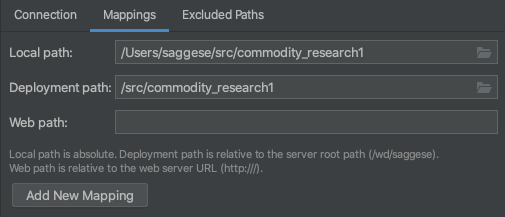
\includegraphics[width=6.5in,height=1.04167in]{media/image10.png}

There are 2 special columns in the by-date file:

\begin{itemize}
\item
  \begin{quote}
  one that represents the timestamp ("start\_time" in the example). This
  is unique and monotonic (start\_time, ticker) are unique
  \end{quote}
\item
  \begin{quote}
  one that represents the asset ("ticker" in the example)
  \end{quote}
\end{itemize}

\textbf{Data stored by-asset.} By-asset data means that there is a
single file for each single asset with the data for all the timestamps
(no timestamp is repeated in a single file)

Bitcoin.pq

1546871400 ...

1546871401

1546871402

Eth.pq

1546871400 ...

1546871401

1546871402

By-asset Parquet data. Data pipelines can transform by-asset data into
Parquet data, preserving all the columns. Successive stages of the
pipeline perform other data transformations. By-asset means that the
asset that is in the innermost directory

```

dst\_dir/

year=2021/

month=12/

day=11/

asset=BTC\_USDT/

data.parquet

asset=ETH\_USDT/

data.parquet

```

Typically the by-date format is just a format that we receive data from,
and we don\textquotesingle t want to transform data to.

The name of the asset can depend on the data and it can be `asset`,
`currency\_pair`, `ticker`.

By default we use names of columns from the data and we reindex the
partitioned dataframe on datetime, so saved parquet will all have the
same datetime index.

Partitioning on year/month/day is optional and should be provided as a
switch in partitioning function.

\textbf{Data stored by-tile.} Data is organized by tile when the Parquet
files are partitioned by asset, by year, and by month so that
it\textquotesingle s possible to read only a chunk of that

asset=BTC\_USDT/

year=2021/

month=12/

data.parquet

year=2021/

month=11/

data.parquet

\ldots{}

asset=ETH\_USDT/

year=2021/

month=12/

data.parquet

\ldots{}

% ===============================================================================
\subsection{Sandbox}

This paragraph describes an example of infrastructure that implements
the Surrentum Data Protocol. The

It is a Docker Container containing the following services:

\begin{itemize}
\item
  \begin{quote}
  Airflow
  \end{quote}
\item
  \begin{quote}
  Jupyter notebook
  \end{quote}
\item
  \begin{quote}
  Postgres
  \end{quote}
\item
  \begin{quote}
  MongoDB
  \end{quote}
\end{itemize}

\textbf{Notes for CK devs (TO REMOVE)}

\begin{itemize}
\item
  \begin{quote}
  It is a separated code base from Surrentum and it shares only a few
  base library (e.g., `helpers`)
  \end{quote}
\item
  \begin{quote}
  It is a scaled down version of CK production infrastructure (e.g.,
  managed Airflow is replaced by a local Airflow instance)
  \end{quote}
\item
  \begin{quote}
  The system follows closely the production system described in
  \href{https://docs.google.com/document/d/1nLhaFBSHVrexCcwJMnpXlkqwn0l6bDiVer34GKVclYY/edit\#}{\ul{Data
  pipelines - Specs}}
  \end{quote}
\end{itemize}

% ===============================================================================
\subsection{Data client stack}

Once the data is downloaded, it needs to be retrieved for processing in
a common format (e.g., DataFlow format).

We use a two layer approach to split the complexity / responsibilities
of reading the data

\begin{itemize}
\item
  \begin{quote}
  `ImClient`
  \end{quote}

  \begin{itemize}
  \item
    \begin{quote}
    Data is downloaded and saved with minimal or no transformation
    \end{quote}
  \item
    \begin{quote}
    Adapts from the vendor data to a standard internal "MarketData"
    format
    \end{quote}
  \end{itemize}
\item
  \begin{quote}
  MarketData` implements "behaviors" that are orthogonal to vendors,
  e.g.,
  \end{quote}

  \begin{itemize}
  \item
    \begin{quote}
    RealTime or Historical
    \end{quote}
  \item
    \begin{quote}
    Stitched (i.e.,"overlap" multiple data sources giving a single view
    of the data). E.g., the data from the last day comes from a
    real-time source while the data before that comes from an historical
    source
    \end{quote}
  \item
    \begin{quote}
    Replayed = serialize the data to disk and read it back, implementing
    also knowledge time as-of-time semantic. This behavior is orthogonal
    to RealTime, Historical, Stitched, i.e., one can replay any
    `MarketData`, including an already replayed one
    \end{quote}
  \end{itemize}
\end{itemize}

\# Data format for `ImClient` / `MarketData` pipeline

- Both `ImClient` and `MarketData` have an output format that is
enforced by the

base and the derived classes together

- `ImClient` and `MarketData` have 3 interfaces each:

1) an external "input" format for a class

- format of the data as input to a class derived from `MarketData` /

`ImClient`

2) an internal "input" format

- format that derived classes need to follow so that the corresponding
base

class can do its job, i.e., apply common transformations to all

`MarketData` / `ImClient` classes

3) an external "output" format

- format of the data outputted by any derived class from `MarketData` /

`ImClient`

- The chain of transformations is:

- Class derived from `ImClient`

- The transformations are vendor-specific

- `ImClient`

- The transformations are fixed

- Class derived from `MarketData`

- The transformations are specific to the `MarketData` concrete class

- `MarketData`

- The transformations are fixed

```plantuml

{[}Vendor{]} -\textgreater{} {[}DerivedImClient{]}

{[}DerivedImClient{]} -\textgreater{} {[}AbstractImClient{]}

{[}AbstractImClient{]} -\textgreater{} {[}DerivedMarketData{]}

{[}DerivedMarketData{]} -\textgreater{} {[}AbstractMarketData{]}

```

\#\# Transformations performed by classes derived from `ImClient`

- Whatever is needed to transform the vendor data into the internal
format accepted

by base `ImClient`

- Only derived classes `ImClient` knows what is exact semantic of the
vendor-data

\#\# Transformations performed by abstract class `ImClient`

- Implemented by `ImClient.\_apply\_im\_normalization()`

\#\# Output format of `ImClient`

- TODO(*): Check the code in `ImClient` since that might be more up to
date than

this document and, if needed, update this doc

- The data in output of a class derived from `ImClient` is normalized so
that:

- the index:

- represents the knowledge time

- is the end of the sampling interval

- is called `timestamp`

- is a tz-aware timestamp in UTC

- the data:

- is resampled on a 1 minute grid and filled with NaN values

- is sorted by index and `full\_symbol`

- is guaranteed to have no duplicates

- belongs to intervals like {[}a, b{]}

- has a `full\_symbol` column with a string representing the canonical
name

of the instrument

- TODO(gp): We are planning to use an `ImClient` data format closer to
`MarketData`

by using `start\_time`, `end\_time`, and `knowledge\_time` since these
can be

inferred only from the vendor data semantic

\#\# Transformations performed by classes derived from `MarketData`

- Classes derived from `MarketData` do whatever they need to do in
`\_get\_data()` to

get the data, but always pass back data that:

- is indexed with a progressive index

- has asset, start\_time, end\_time, knowledge\_time

- start\_time, end\_time, knowledge\_time are timezone aware

- E.g.,

```

asset\_id start\_time end\_time close volume

idx

0 17085 2021-07-26 13:41:00+00:00 2021-07-26 13:42:00+00:00 148.8600
400176

1 17085 2021-07-26 13:30:00+00:00 2021-07-26 13:31:00+00:00 148.5300
1407725

2 17085 2021-07-26 13:31:00+00:00 2021-07-26 13:32:00+00:00 148.0999
473869

```

\#\# Transformations performed by abstract class `MarketData`

- The transformations are done inside `get\_data\_for\_interval()`,
during normalization,

and are:

- indexing by `end\_time`

- converting `end\_time`, `start\_time`, `knowledge\_time` to the
desired timezone

- sorting by `end\_time` and `asset\_id`

- applying column remaps

\#\# Output format of `MarketData`

- The base `MarketData` normalizes the data by:

- sorting by the columns that correspond to `end\_time` and `asset\_id`

- indexing by the column that corresponds to `end\_time`, so that it is
suitable

to DataFlow computation

- E.g.,

```

asset\_id start\_time close volume

end\_time

2021-07-20 09:31:00-04:00 17085 2021-07-20 09:30:00-04:00 143.990
1524506

2021-07-20 09:32:00-04:00 17085 2021-07-20 09:31:00-04:00 143.310 586654

2021-07-20 09:33:00-04:00 17085 2021-07-20 09:32:00-04:00 143.535 667639

```

\# Asset ids format

- `ImClient` uses assets encoded as `full\_symbols` strings (e.g.,
`binance::BTC\_UTC`)

- There is a vendor-specific mapping:

- from `full\_symbols` to corresponding data

- from `asset\_ids` (ints) to `full\_symbols` (strings)

- If the `asset\_ids` -\textgreater{} `full\_symbols` mapping is
provided by the vendor, then we

reuse it

- Otherwise, we build a mapping hashing `full\_symbols` strings into
numbers

- `MarketData` and everything downstream uses `asset\_ids` that are
encoded as ints

- This is because we want to use ints and not strings in dataframe

\# Handling of `asset\_ids`

- Different implementations of `ImClient` backing a `MarketData` are
possible,

e.g.:

- The caller needs to specify the requested `asset\_ids`

- In this case the universe is provided by `MarketData` when calling the

data access methods

- The reading backend is initialized with the desired universe of assets
and

then `MarketData` just uses or subsets that universe

- For these reasons, assets are selected at 3 different points:

1) `MarketData` allows to specify or subset the assets through
`asset\_ids`

through the constructor

2) `ImClient` backends specify the assets returned

- E.g., a concrete implementation backed by a DB can stream the data for

its entire available universe

3) Certain class methods allow querying data for a specific asset or
subset

of assets

- For each stage, a value of `None` means no filtering

\# Handling of filtering by time

- Clients of `MarketData` might want to query data by:

- using different interval types, namely `{[}a, b), {[}a, b{]}, (a,
b{]}, (a, b)`

- filtering on either the `start\_ts` or `end\_ts`

- For this reason, this class supports all these different ways of
providing data

- `ImClient` has a fixed semantic of the interval `{[}a, b{]}`

- `MarketData` adapts the fixed semantic to multiple ones

\# Handling timezone

- `ImClient` always uses UTC as output

- `MarketData` adapts UTC to the desired timezone, as requested by the
client

\hypertarget{checklist-for-releasing-a-new-data-set}{%
\subsection{\#\# Checklist for releasing a new data
set}\label{checklist-for-releasing-a-new-data-set}}

\begin{itemize}
\item
  \begin{quote}
  Decide what to do exactly (e.g., do we download only bulk data or also
  real-time?)
  \end{quote}
\item
  \begin{quote}
  Review what code we have and what can be generalized to accomplish the
  task at hand
  \end{quote}
\item
  \begin{quote}
  Decide what\textquotesingle s the name of the data set according to
  our convention
  \end{quote}
\item
  \begin{quote}
  Create DAGs for Airflow
  \end{quote}
\item
  \begin{quote}
  Update the Raw Data Gallery
  im\_v2/common/notebooks/Master\_raw\_data\_gallery.ipynb
  \end{quote}
\item
  \begin{quote}
  Quick exploratory analysis to make sure the data is not malformed
  \end{quote}
\item
  \begin{quote}
  Update the table in
  \href{https://docs.google.com/document/d/1nLhaFBSHVrexCcwJMnpXlkqwn0l6bDiVer34GKVclYY/edit\#heading=h.8g5ajvlq6zks}{\ul{Data
  pipelines - Specs}}
  \end{quote}
\item
  \begin{quote}
  Exploratory analysis for a thorough QA analysis
  \end{quote}
\item
  \begin{quote}
  Add QA system to Airflow prod
  \end{quote}
\end{itemize}

\hypertarget{surrentum-node-specification}{%
\section{\# Surrentum Node:
specification}\label{surrentum-node-specification}}

\hypertarget{time-semantics}{%
\subsection{\#\# Time semantics}\label{time-semantics}}

\textbf{Time semantics}. A Surrentum component can be executed or
simulated accounting for different ways to represent the passing of
time. E.g., it can be simulated in a timed or non-timed simulation,
depending on how data is delivered to the system (as it is generated or
in bulk with knowledge time).

\textbf{Clock.} A function that reports the current timestamp. There are
3 versions of clock:

\begin{enumerate}
\def\labelenumi{\arabic{enumi})}
\item
  \begin{quote}
  Static clock. A clock that remains the same during a system run.
  \end{quote}

  \begin{enumerate}
  \def\labelenumii{\alph{enumii}.}
  \item
    \begin{quote}
    Future peeking is allowed
    \end{quote}
  \end{enumerate}
\item
  \begin{quote}
  Replayed clock. A moving clock that can be in the past or future with
  respect to a real clock
  \end{quote}

  \begin{enumerate}
  \def\labelenumii{\alph{enumii}.}
  \item
    \begin{quote}
    Use time passing at the same pace of real-time wall-clock or
    \end{quote}
  \item
    \begin{quote}
    Simulate time based on events, e.g., as soon as the workload
    corresponding to one timestamp is complete we move to the next
    timestamp, without waiting for the actual time to pass
    \end{quote}
  \item
    \begin{quote}
    Future peeking is technically possible but is prohibited
    \end{quote}
  \end{enumerate}
\item
  \begin{quote}
  Real clock. The wall-clock time matches what we observe in real-life,
  data is provided to processing units as it is produced by systems.
  \end{quote}

  \begin{enumerate}
  \def\labelenumii{\alph{enumii}.}
  \item
    \begin{quote}
    Future peeking is not possible in principle
    \end{quote}
  \end{enumerate}
\end{enumerate}

\textbf{Knowledge time.} It is the time when data becomes available
(e.g., downloaded or computed) to a system. Each row of data is tagged
with the corresponding knowledge time. Data with knowledge time after
the current clock time must not be observable in order to avoid future
peeking.

\textbf{Timed simulation}. Sometimes referred to as historical,
vectorized, bulk, batch simulation. In a timed simulation the data is
provided with a clock that reports the current timestamp. Data with
knowledge time after the current timestamp must not be observable in
order to avoid future peeking.

TODO(gp): Add an example of df with forecasts explaining the timing

\textbf{Non-timed simulation}. (Sometimes referred to as event-based,
reactive simulation). Clock type is ``static clock''. Typically
wall-clock time is a timestamp that corresponds to the latest knowledge
time (or greater) in a dataframe. In this way all data in a dataframe is
available because every row has a knowledge time that is less than or
equal to the wall-clock time. Note that the clock is static, i.e. not
moving. In a non-timed simulation, the data is provided in a dataframe
for the entire period of interest.

E.g., for a system predicting every 5 mins, all the input data are
equally spaced on a 5-min grid and indexed with knowledge time.

TODO(gp): Add an example of df with forecasts explaining the timing

df{[}"c"{]} = (df{[}"a"{]} + df{[}"b"{]}).shift(1)

\textbf{Real-time execution}. In real-time the clock type is ``real
clock''.

E.g., for a system predicting every 5 mins, one forecast is delivered
every 5 mins of wall-clock.

\# TODO(Grisha): add an example.

\textbf{Replayed simulation}. In replayed simulation, the data is
provided in the same "format" and with the same timing than it would be
provided in real-time, but the clock type is ``replayed clock''.

TODO(gp): Add an example of df with forecasts explaining the timing

\hypertarget{different-views-of-system-components}{%
\subsection{\#\# Different views of System
components}\label{different-views-of-system-components}}

\textbf{Different implementations of a component}. A Surrentum component
is described in terms of an interface and can have several
implementations at different levels of detail.

\textbf{Reference implementation}. A reference implementation is
vendor-agnostic implementation of a component (e.g., DataFrameImClient,
DataFrameBroker)

\textbf{Vendor implementation}. A vendor implementation is a
vendor-specific implementation of a component (e.g., CcxtImClient,
CcxtBroker).

\textbf{Mocked implementation}. A mocked implementation is a simulated
version of a vendor-specific component (e.g., a DataFrameCcxtBroker). A
mocked component can have the same timing semantics as the
real-component (e.g., an asynchronous or reactive implementation) or
not.

\hypertarget{architecture}{%
\subsection{\#\# Architecture}\label{architecture}}

In this section we summarize the responsibilities and the high level
invariants of each component of a `System`.

The entire System is represented in terms of a Config. Each piece of a
Config refers to and configures a specific part of the System. Each
component should be completely configured in terms of a Config.

\hypertarget{component-invariants}{%
\subsubsection{\#\#\# Component invariants}\label{component-invariants}}

Each component has a way to know:

\begin{itemize}
\item
  \begin{quote}
  what is the current time (e.g., the real-time machine time or the
  simulated one)
  \end{quote}
\item
  \begin{quote}
  the timestamp of the current data bar it\textquotesingle s working on
  \end{quote}
\end{itemize}

All data in components should be indexed by the knowledge time (i.e.,
when the data became available to that component) in terms of current
time.

Each component should print its state so that one can inspect how
exactly it has been initialized.

Each component can be serialized and deserialized from disk.

Each component can be mocked for simulating.

Each component should save data in a directory as it executes to make
the system observable.

Models are described in terms of DAGs using the DataFlowCompute
framework

\textbf{Misc}. Models read data from historical and real-time data sets,
typically not mixing these two styles.

Raw data is typically stored in S3 bucket in the same format as it comes
or in Parquet format.

\hypertarget{config}{%
\subsection{\#\# Config}\label{config}}

\textbf{Config}. A `Config` is a dictionary-like object that represents
parameters used to build and configure other objects (e.g., a DAG or a
System).

Each config is a hierarchical structure which consists of
\textbf{Subconfigs} and \textbf{Leaves}.

\textbf{Subconfig} is a nested object which represents a Config inside
another config. A Subconfig of a Subconfig is a Subconfig of a Config,
i.e. the relation is transitive.

\textbf{Leaf} is any object inside a Config that is used to build
another object that is not in itself a Config.

Note that a dictionary or other mapping objects are not permitted inside
a Config: each dictionary-like object should be converted to a Config
and become a Subconfig.

\hypertarget{config-representation-and-properties}{%
\subsubsection{\#\#\# Config representation and
properties}\label{config-representation-and-properties}}

A Config can be represented as a dictionary or a string.

Example of a dictionary representation:

```

config1 = \{

"resample\_1min": False,

"client\_config": \{

"universe": \{

"full\_symbols": {[}"binance::ADA\_USDT"{]},

"universe\_version": "v3",

\},

\},

"market\_data\_config": \{"start\_ts": start\_ts, "end\_ts": end\_ts\},

\}

```

In the example above:

\begin{itemize}
\item
  \begin{quote}
  ``resample\_1min'' is a leaf of the `config1`
  \end{quote}
\item
  \begin{quote}
  ``client\_config'' is a subconfig of `config1`
  \end{quote}
\item
  \begin{quote}
  ``universe'' is a subconfig of ``client\_config''
  \end{quote}
\item
  \begin{quote}
  ``market\_data'' config is a subconfig of ``config1''
  \end{quote}
\item
  \begin{quote}
  ``start\_ts'' and ``end\_ts'' are leaves of ``market\_data\_config''
  and `config1`
  \end{quote}
\end{itemize}

Example of a string representation:

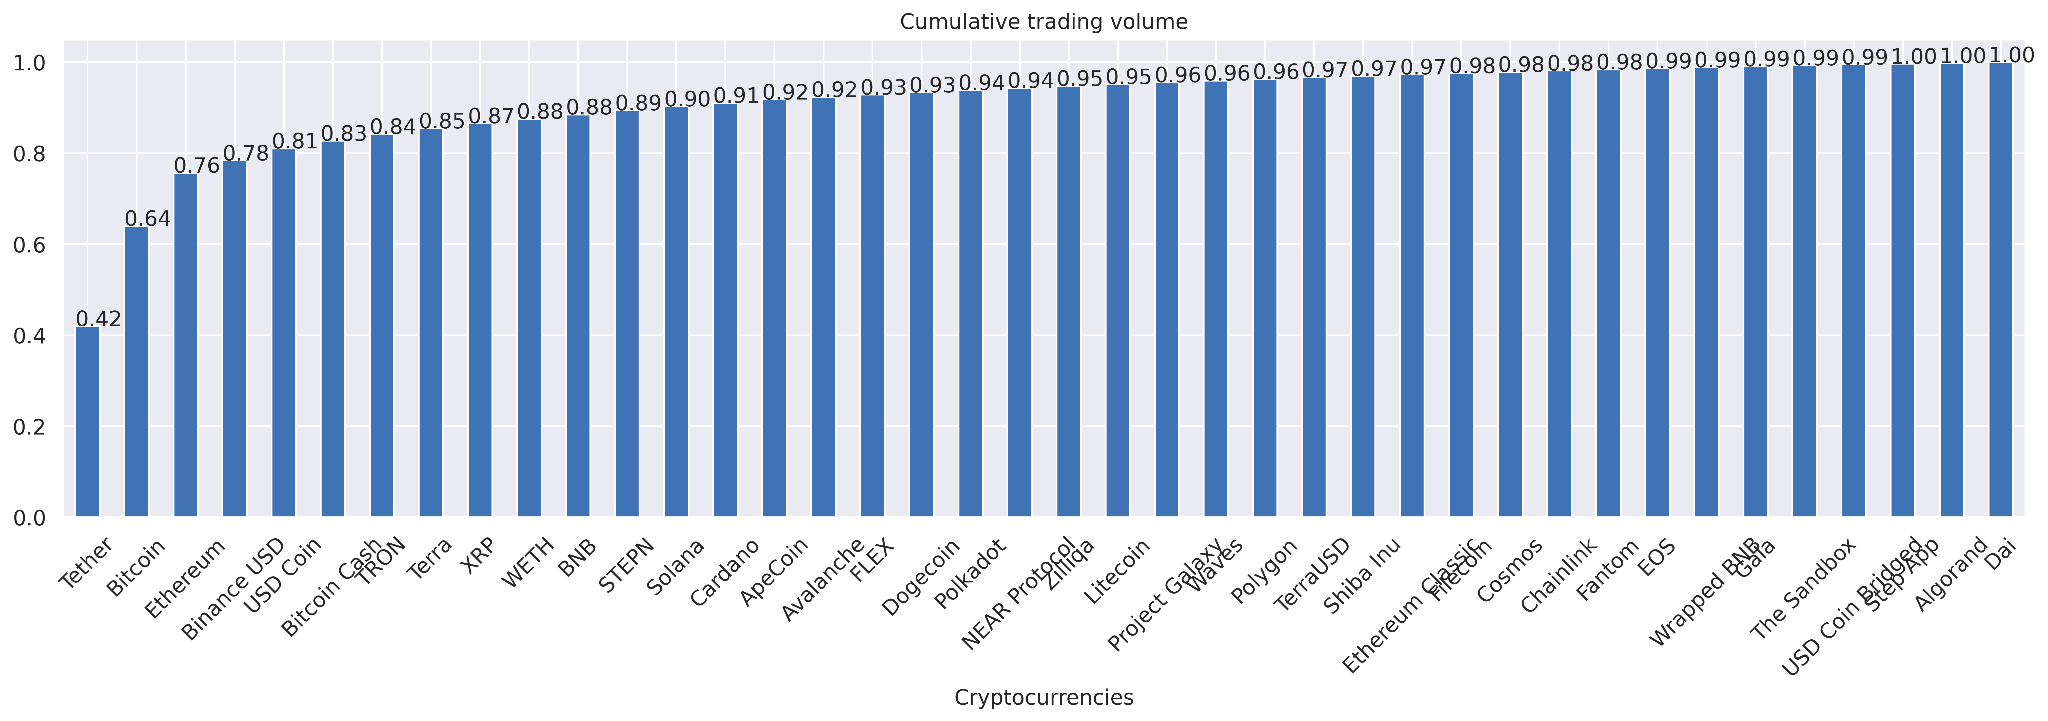
\includegraphics[width=6.85478in,height=1.23034in]{media/image11.png}

\begin{itemize}
\item
  \begin{quote}
  The same values are annotated with `marked\_as\_used`, `writer` and
  `val\_type`
  \end{quote}

  \begin{itemize}
  \item
    \begin{quote}
    `marked\_as\_used` determines whether the object was used to
    construct another object
    \end{quote}
  \item
    \begin{quote}
    `writer` provides a stacktrace of the piece of code which marked the
    object as used
    \end{quote}
  \item
    \begin{quote}
    `val\_type` is a type of the object
    \end{quote}
  \end{itemize}
\end{itemize}

\hypertarget{assigning-and-getting-config-items}{%
\subsubsection{\#\#\# Assigning and getting Config
items}\label{assigning-and-getting-config-items}}

\begin{itemize}
\item
  \begin{quote}
  Config object has its own implementations of `\_\_setitem\_\_` and
  `\_\_getitem\_\_`
  \end{quote}
\item
  \begin{quote}
  A new value can be set freely like in a python Dict object
  \end{quote}
\item
  \begin{quote}
  Overwriting the value is prohibited if the value has already been used
  \end{quote}
\end{itemize}

Since Config is used to guarantee that the construction of any objects
is reproducible, there are 2 methods to `get` the value.

\begin{itemize}
\item
  \begin{quote}
  `get\_and\_mark\_as\_used` is utilized when a leaf of the config is
  used to construct another object
  \end{quote}

  \begin{itemize}
  \item
    \begin{quote}
    When the value is used inside a constructor
    \end{quote}
  \item
    \begin{quote}
    When the value is used as a parameter in a function
    \end{quote}
  \end{itemize}
\end{itemize}

Note that when selecting a subconfig the subconfig itself is not marked
as used, but its leaves are. For this reason, the user should avoid
marking subconfigs as used and instead select leaves separately.

Example of marking the subconfig as used:

```

\_ = config.get\_and\_mark\_as\_used(``market\_data\_config'')

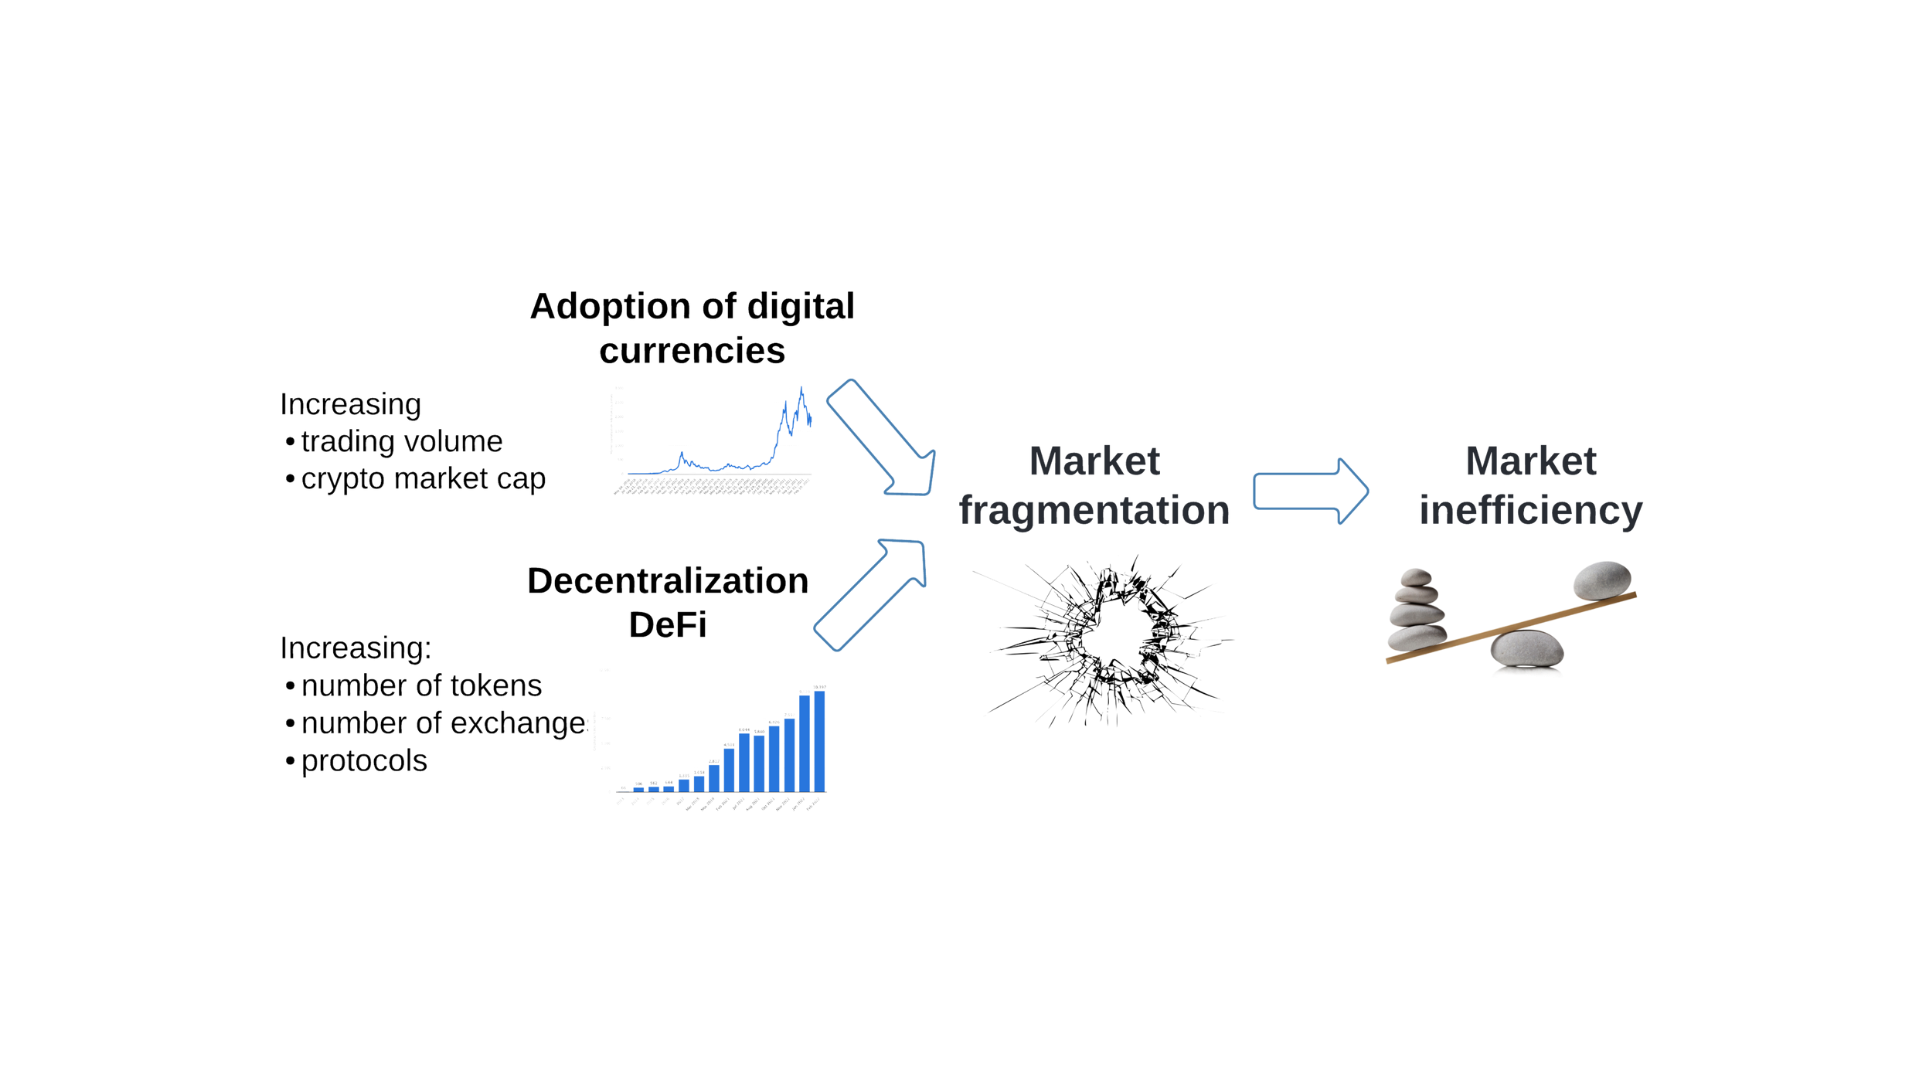
\includegraphics[width=6.5in,height=1.19444in]{media/image12.png}

```

Example of marking the leaf as used:

```

\_ = config.get\_and\_mark\_as\_used(("market\_data\_config",
"end\_ts"))

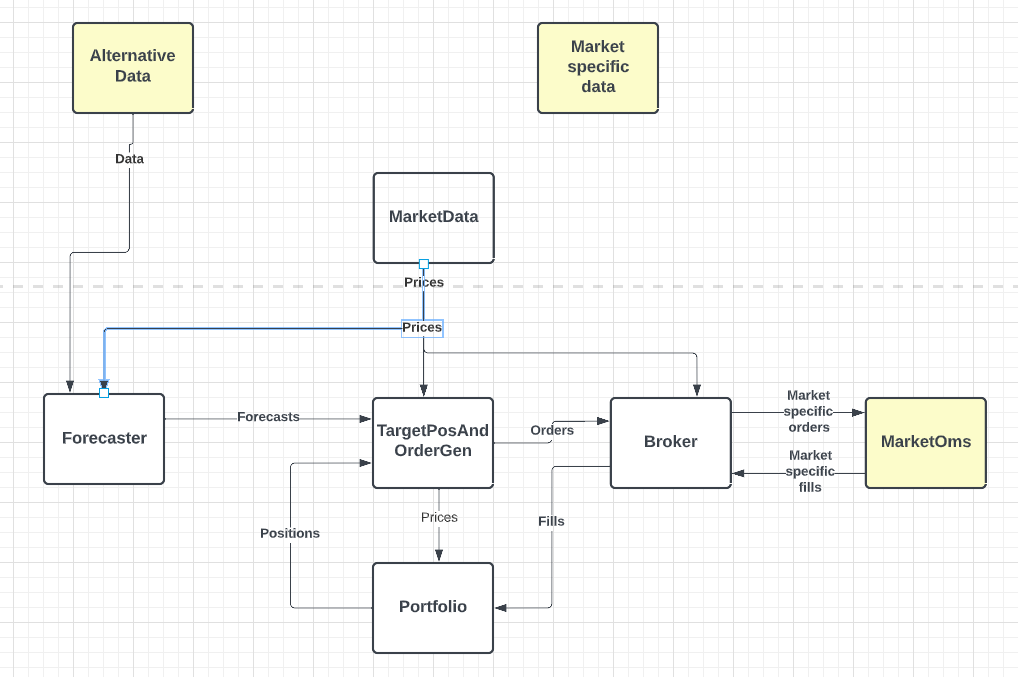
\includegraphics[width=6.5in,height=1.13889in]{media/image15.png}

```

\begin{itemize}
\item
  \begin{quote}
  `\_\_getitem\_\_` is used to select items for uses which do not affect
  the construction of other objects:
  \end{quote}

  \begin{itemize}
  \item
    \begin{quote}
    Logging, debugging and printing
    \end{quote}
  \end{itemize}
\end{itemize}

\hypertarget{dataflow-computing}{%
\subsection{\#\# DataFlow computing}\label{dataflow-computing}}

\begin{itemize}
\item
  \begin{quote}
  \textbf{DataFlow framework}. DataFlow is a computing framework to
  implement machine learning models that can run with minimal changes in
  timed, non-timed, replayed simulation and real-time execution.
  \end{quote}
\end{itemize}

The working principle underlying DataFlow is to run a model in terms of
time slices of data so that both historical and real-time semantics can
be accommodated without changing the model.

TODO(gp): Explain the advantages:

\begin{itemize}
\item
  \begin{quote}
  Tiling to fit in memory
  \end{quote}
\item
  \begin{quote}
  Cached computation
  \end{quote}
\item
  \begin{quote}
  Adapt a procedural semantic to a reactive / streaming semantic
  \end{quote}
\item
  \begin{quote}
  Handle notion of time
  \end{quote}
\item
  \begin{quote}
  Control for future peeking
  \end{quote}
\item
  \begin{quote}
  Suite of tools to replay and debug executions from real-time
  \end{quote}
\item
  \begin{quote}
  Support for market data and other tabular data feeds
  \end{quote}
\item
  \begin{quote}
  Support for knowledge time
  \end{quote}
\end{itemize}

\# Resampling VWAP (besides potential errors). This implies hardcoded
formula in a mix with resampling functions.

vwap\_approach\_2 = (converted\_data{[}"close"{]} *
converted\_data{[}"volume"{]}).resample(

resampling\_freq

).mean() /
converted\_data{[}"volume"{]}.resample(resampling\_freq).sum()

vwap\_approach\_2.head(3)

\textbf{Dag Node}. It is a unit of computation of a DataFlow model. A
Dag node has inputs, outputs, a unique node id (aka `nid`), and a state.
Typically inputs and outputs are dataframes. A Dag node stores a value
for each output and method name (e.g., methods are `fit`, `predict`,
`save\_state`, `load\_state`). The DataFlow time slice semantics is
implemented in terms of `Pandas` and `Sklearn` libraries.

TODO(gp): Add picture.

\textbf{DataFlow model}. A DataFlow model (aka `DAG`) is a direct
acyclic graph composed of DataFlow nodes. It allows to connect, query
the structure

Running a method on a Dag means running that method on all its nodes in
topological order, propagating values through the Dag nodes.

TODO(gp): Add picture.

\textbf{DagConfig}. A `Dag` can be built assembling Nodes using a
function representing the connectivity of the nodes and parameters
contained in a Config (e.g., through a call to a builder
`DagBuilder.get\_dag(config)`).

A DagConfig is hierarchical and contains one subconfig per Dag node. It
should only include `Dag` node configuration parameters, and not
information about `Dag` connectivity, which is specified in the `Dag`
builder part.

\hypertarget{template-configs}{%
\subsubsection{\texorpdfstring{\textbf{Template
configs}}{Template configs}}\label{template-configs}}

\begin{itemize}
\item
  \begin{quote}
  Are incomplete configs, with some "mandatory" parameters unspecified
  but clearly identified with `cconfig.DUMMY` value
  \end{quote}
\item
  \begin{quote}
  Have reasonable defaults for specified parameters
  \end{quote}

  \begin{itemize}
  \item
    \begin{quote}
    This facilitates config extension (e.g., if we add additional
    parameters / flexibility in the future, then we should not have to
    regenerate old configs)
    \end{quote}
  \end{itemize}
\item
  \begin{quote}
  Leave dummy parameters for frequently-varying fields, such as `ticker`
  \end{quote}
\item
  \begin{quote}
  Should be completable and be completed before use
  \end{quote}
\item
  \begin{quote}
  Should be associated with a `Dag` builder
  \end{quote}
\end{itemize}

\textbf{DagBuilder}. It is an object that builds a DAG and has a
`get\_config\_template()` and a `get\_dag()` method to keep the config
and the Dag in sync.

The client:

\begin{itemize}
\item
  \begin{quote}
  calls `get\_config\_template()` to receive the template config
  \end{quote}
\item
  \begin{quote}
  fills / modifies the config
  \end{quote}
\item
  \begin{quote}
  uses the final config to call `get\_dag(config)` and get a fully built
  DAG
  \end{quote}
\end{itemize}

A `DagBuilder` can be passed to other objects instead of `Dag` when the
template config is fully specified and thus the `Dag` can be constructed
from it.

\textbf{DagRunner}. It is an object that allows to run a `Dag`.
Different implementations of a `DagRunner` allow to run a `Dag` on data
in different ways, e.g.,

\begin{itemize}
\item
  \begin{quote}
  `FitPredictDagRunner`: implements two methods `fit` / `predict` when
  we want to learn on in-sample data and predict on out-of-sample data
  \end{quote}
\item
  \begin{quote}
  `RollingFitPredictDagRunner`: allows to fit and predict on some data
  using a rolling pattern
  \end{quote}
\item
  \begin{quote}
  `IncrementalDagRunner`: allows to run one step at a time like in
  real-time
  \end{quote}
\item
  \begin{quote}
  `RealTimeDagRunner`: allows to run using nodes that have a real-time
  semantic
  \end{quote}
\end{itemize}

\hypertarget{dataflow-computation-semantics}{%
\subsection{\#\# DataFlow Computation
Semantics}\label{dataflow-computation-semantics}}

Often raw data is available in a "long format", where the data is
conditioned on the asset (e.g., full\_symbol), e.g.,

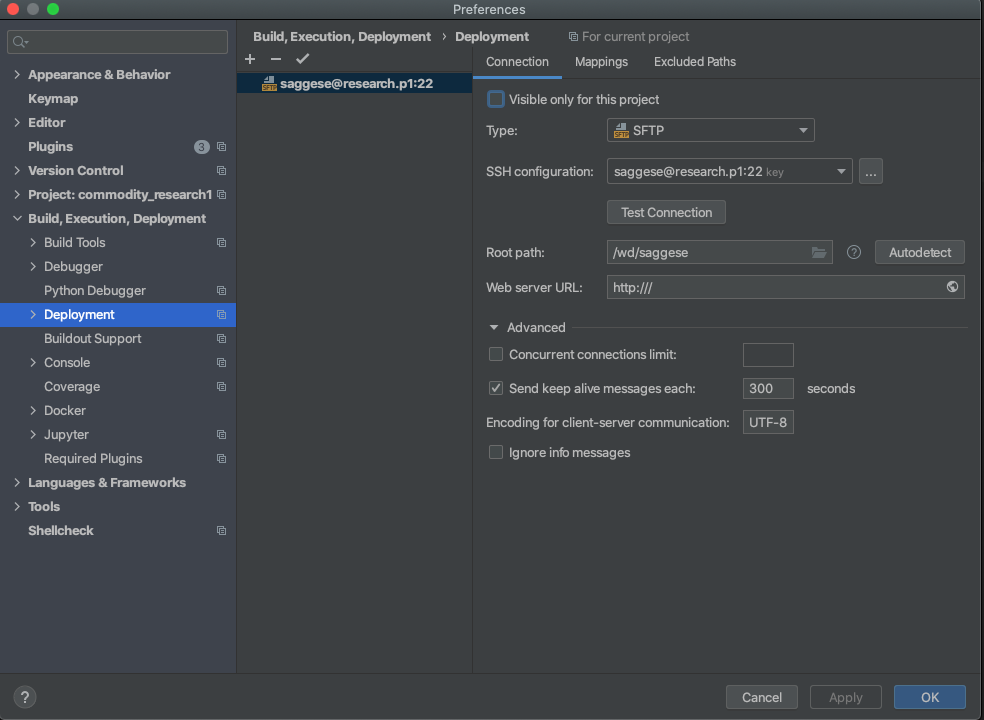
\includegraphics[width=5.33854in,height=1.10364in]{media/image3.png}

DataFlow represents data through multi-index dataframes, where

\begin{itemize}
\item
  \begin{quote}
  the outermost index is the "feature"
  \end{quote}
\item
  \begin{quote}
  the innermost index is the asset, e.g.,
  \end{quote}
\end{itemize}

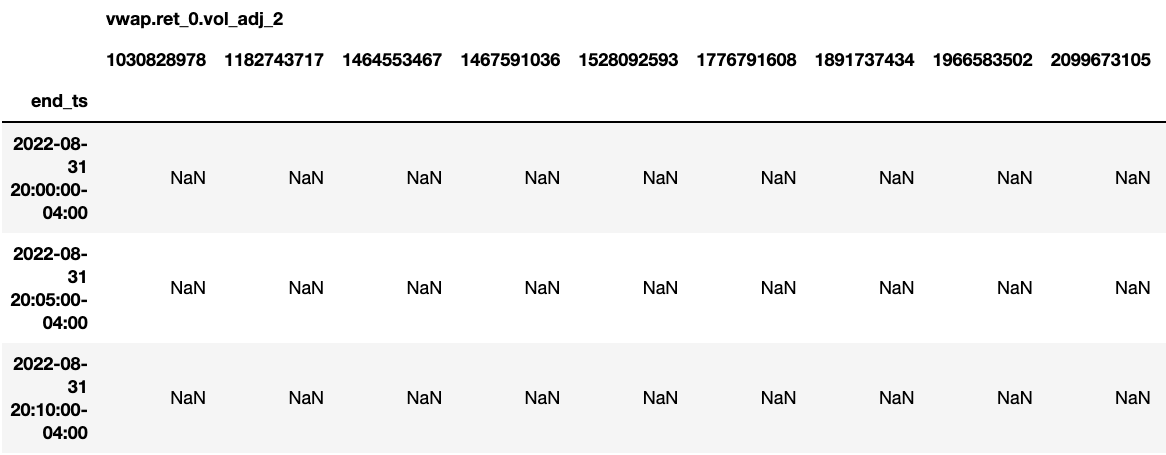
\includegraphics[width=6.5in,height=1.04167in]{media/image8.png}

The reason for this convention is that typically features are computed
in an univariate fashion (e.g., asset by asset), and we can get
vectorization over the assets by expressing operations in terms of the
features. E.g., we can express a feature as `(df{[}"close",
"open"{]}.max() - df{[}"high"{]}).shift(2)`.

Based on the example
./amp/dataflow/notebooks/gallery\_dataflow\_example.ipynb, one can work
with DataFlow at 4 levels of abstraction:

\begin{enumerate}
\def\labelenumi{\arabic{enumi})}
\item
  \begin{quote}
  Pandas long-format (non multi-index) dataframes and for-loops
  \end{quote}

  \begin{itemize}
  \item
    \begin{quote}
    We can do a group-by or filter by full\_symbol
    \end{quote}
  \item
    \begin{quote}
    Apply the transformation on each resulting df
    \end{quote}
  \item
    \begin{quote}
    Merge the data back into a single dataframe with the long-format
    \end{quote}
  \end{itemize}
\item
  \begin{quote}
  Pandas multiindex dataframes
  \end{quote}

  \begin{itemize}
  \item
    \begin{quote}
    The data is in the DataFlow native format
    \end{quote}
  \item
    \begin{quote}
    We can apply the transformation in a vectorized way
    \end{quote}
  \item
    \begin{quote}
    This approach is best for performance and with compatibility with
    DataFlow point of view
    \end{quote}
  \item
    \begin{quote}
    An alternative approach is to express multi-index transformations in
    terms of approach 1 (i.e., single asset transformations and then
    concatenation). This approach is functionally equivalent to a
    multi-index transformation, but typically slow and memory
    inefficient
    \end{quote}
  \end{itemize}
\item
  \begin{quote}
  DataFlow nodes
  \end{quote}

  \begin{itemize}
  \item
    \begin{quote}
    A node implements a certain transformations on DataFrames according
    to the DataFlow convention and interfaces
    \end{quote}
  \item
    \begin{quote}
    Nodes operate on the multi-index representation by typically calling
    functions from level 2 above
    \end{quote}
  \end{itemize}
\item
  \begin{quote}
  DAG
  \end{quote}

  \begin{itemize}
  \item
    \begin{quote}
    A series of transformations in terms of DataFlow nodes
    \end{quote}
  \end{itemize}
\end{enumerate}

Note that there are degrees of freedom in splitting the work between the
various layers.

E.g., code can be split in multiple functions at level 2) and then

\href{http://172.30.2.136:10051/notebooks/dataflow_orange/pipelines/C1/notebooks/C1b_debugging.ipynb}{\ul{http://172.30.2.136:10051/notebooks/dataflow\_orange/pipelines/C1/notebooks/C1b\_debugging.ipynb}}

\href{http://172.30.2.136:10051/notebooks/dataflow_orange/pipelines/C1/notebooks/Implement_RH1E.ipynb}{\ul{http://172.30.2.136:10051/notebooks/dataflow\_orange/pipelines/C1/notebooks/Implement\_RH1E.ipynb}}

\hypertarget{backtest-and-experiment}{%
\subsection{\#\# Backtest and
Experiment}\label{backtest-and-experiment}}

\hypertarget{configbuilder}{%
\subsubsection{\texorpdfstring{\textbf{\#\#\#
`ConfigBuilder`}}{\#\#\# `ConfigBuilder`}}\label{configbuilder}}

\begin{itemize}
\item
  \begin{quote}
  Generates a list of fully formed (not template) configs that can be
  then run
  \end{quote}
\item
  \begin{quote}
  These configs can correspond to one or multiple Experiments, tiled or
  not (see below)
  \end{quote}
\item
  \begin{quote}
  Config builder accepts `BacktestConfig` as an input
  \end{quote}
\end{itemize}

\hypertarget{experiment-in-strict-and-loose-sense}{%
\subsubsection{\texorpdfstring{\textbf{\#\#\# Experiment in strict and
loose
sense}}{\#\#\# Experiment in strict and loose sense}}\label{experiment-in-strict-and-loose-sense}}

Colloquially, we use experiment to mean different things, e.g., an
experiment can consists in:

\begin{itemize}
\item
  \begin{quote}
  a backtest where we run a single Dag with a single config (e.g., when
  we test the predictive power of a single model)
  \end{quote}
\end{itemize}

\begin{itemize}
\item
  \begin{quote}
  running a Dag (e.g., E8d) through multiple configs (e.g., with longer
  / shorter history) to perform an "A / B experiment"
  \end{quote}
\item
  \begin{quote}
  running completely different Dags (e.g., E1 vs E8c) to compare their
  performance
  \end{quote}
\end{itemize}

Strictly speaking, we refer to:

\begin{itemize}
\item
  \begin{quote}
  The first one as a `Backtest` (which can be executed in terms of tiled
  configs or not)
  \end{quote}
\item
  \begin{quote}
  The second and the third as an `Experiment`
  \end{quote}
\end{itemize}

In practice almost any experiment we run consists of one or more
backtests

\hypertarget{backtest}{%
\subsubsection{\texorpdfstring{\textbf{\#\#\#
`Backtest`}}{\#\#\# `Backtest`}}\label{backtest}}

\begin{itemize}
\item
  \begin{quote}
  In general a "backtest" is simply code that is configured by a
  *single* `Config`s
  \end{quote}

  \begin{itemize}
  \item
    \begin{quote}
    The code contained in a backtest experiment can be anything
    \end{quote}
  \end{itemize}
\end{itemize}

\begin{itemize}
\item
  \begin{quote}
  Typically a backtest consists of:
  \end{quote}

  \begin{itemize}
  \item
    \begin{quote}
    creating a `Dag`(e.g., through a `DagBuilder`) or a `System` based
    on a config
    \end{quote}
  \item
    \begin{quote}
    running it over a period of time (e.g., through a `DagRunner`)
    \end{quote}
  \item
    \begin{quote}
    saving the result into a directory
    \end{quote}
  \end{itemize}
\end{itemize}

\hypertarget{backtestconfig}{%
\subsubsection{\texorpdfstring{\textbf{\#\#\#
`BacktestConfig`}}{\#\#\# `BacktestConfig`}}\label{backtestconfig}}

\begin{itemize}
\item
  \begin{quote}
  = a config that has multiple parts configuring both what to run (e.g.,
  a `Dag`) and how to run it (e.g., the universe, the period of time)
  \end{quote}
\item
  \begin{quote}
  It can correspond to multiple configs (e.g., when running a
  `TiledBacktest`)
  \end{quote}
\item
  \begin{quote}
  The common pattern is
  `\textless universe\textgreater-\textless top\_n\textgreater.\textless trading\_period\textgreater.\textless time\_interval\textgreater`,
  e.g., `ccxt\_v4-top3.5T.2019\_2022` where
  \end{quote}

  \begin{itemize}
  \item
    \begin{quote}
    `ccxt\_v4` is a specific version of universe
    \end{quote}
  \item
    \begin{quote}
    `top3` is top 3 assets, `all` means all assets in the universe
    \end{quote}
  \item
    \begin{quote}
    `5T` (5 minutes) is trading period
    \end{quote}
  \item
    \begin{quote}
    `2019-2022` is timeframe, i.e. run the model using data from 2019 to
    2022
    \end{quote}
  \end{itemize}
\end{itemize}

\hypertarget{experiment}{%
\subsubsection{\texorpdfstring{\textbf{\#\#\#
`Experiment`}}{\#\#\# `Experiment`}}\label{experiment}}

\begin{itemize}
\item
  \begin{quote}
  A set of backtests to run, each of which corresponds to conceptually a
  single `Config`
  \end{quote}
\item
  \begin{quote}
  Each backtest can then be executed in a tiled fashion (e.g., by
  expressing it in terms of different configs, one per tile
  \end{quote}
\end{itemize}

In order to create the list of fully built configs, both a `Backtest`
and a `Experiment` need:

\begin{itemize}
\item
  \begin{quote}
  an `BacktestBuilder` (what to run in a backtest)
  \end{quote}
\item
  \begin{quote}
  a `ConfigBuilder` (how to configure)
  \end{quote}
\item
  \begin{quote}
  dst\_dir (destination dir of the entire experiment list, i.e., the one
  that the user passes to the command)
  \end{quote}
\end{itemize}

\hypertarget{tiled-backtest-experiment}{%
\subsubsection{\texorpdfstring{\textbf{\#\#\# Tiled backtest /
experiment}}{\#\#\# Tiled backtest / experiment}}\label{tiled-backtest-experiment}}

\begin{itemize}
\item
  \begin{quote}
  An experiment / backtest that is run through multiple tiles for time
  and assets
  \end{quote}
\item
  \begin{quote}
  In general this is just an implementation detail
  \end{quote}
\end{itemize}

\hypertarget{tiled-vs-tile}{%
\subsubsection{\texorpdfstring{\textbf{\#\#\# Tiled vs
Tile}}{\#\#\# Tiled vs Tile}}\label{tiled-vs-tile}}

\begin{itemize}
\item
  \begin{quote}
  We call "tiled" objects that are split in tiles (e.g.,
  `TiledBacktest`), and "tile" objects that refer to tiling (e.g.,
  `TileConfig`)
  \end{quote}
\end{itemize}

\hypertarget{experiment-list-manager}{%
\subsubsection{\texorpdfstring{\textbf{\#\#\# Experiment (list)
manager}}{\#\#\# Experiment (list) manager}}\label{experiment-list-manager}}

\begin{itemize}
\item
  \begin{quote}
  TODO(gp): experiment\_list manager?
  \end{quote}
\item
  \begin{quote}
  Python code that runs experiments by:
  \end{quote}

  \begin{itemize}
  \item
    \begin{quote}
    generating a list of `Config` object to run, based on a
    `ConfigBuilder` (i.e., `run\_experiment.py` and `run\_notebook.py`)
    \end{quote}
  \end{itemize}
\end{itemize}

\hypertarget{experimentbuilder}{%
\subsubsection{\texorpdfstring{\textbf{\#\#\#
`ExperimentBuilder`}}{\#\#\# `ExperimentBuilder`}}\label{experimentbuilder}}

\begin{itemize}
\item
  \begin{quote}
  TODO(gp): -\textgreater{} BacktestBuilder
  \end{quote}
\item
  \begin{quote}
  It is a function that:
  \end{quote}

  \begin{itemize}
  \item
    \begin{quote}
    Creates a DAG from the passed config
    \end{quote}
  \item
    \begin{quote}
    Runs the DAG
    \end{quote}
  \item
    \begin{quote}
    Saves the results in a specified directory
    \end{quote}
  \end{itemize}
\end{itemize}

\hypertarget{backtestrunner}{%
\subsubsection{\texorpdfstring{\textbf{\#\#\#
`BacktestRunner`}}{\#\#\# `BacktestRunner`}}\label{backtestrunner}}

\begin{itemize}
\item
  \begin{quote}
  A test case object that:
  \end{quote}

  \begin{itemize}
  \item
    \begin{quote}
    runs a backtest (experiment) on a Dag and a Config
    \end{quote}
  \item
    \begin{quote}
    processes its results (e.g., check that the output is readable,
    extract a PnL curve or other statistics)
    \end{quote}
  \end{itemize}
\end{itemize}

\hypertarget{system}{%
\subsubsection{\texorpdfstring{\textbf{\#\#\#
System}}{\#\#\# System}}\label{system}}

\begin{itemize}
\item
  \begin{quote}
  An object representing a full trading system comprising of:
  \end{quote}

  \begin{itemize}
  \item
    \begin{quote}
    MarketData
    \end{quote}

    \begin{itemize}
    \item
      \begin{quote}
      HistoricalMarketData (ImClient)
      \end{quote}
    \item
      \begin{quote}
      RealTimeMarketData
      \end{quote}
    \end{itemize}
  \item
    \begin{quote}
    Dag
    \end{quote}
  \item
    \begin{quote}
    DagRunner
    \end{quote}
  \item
    \begin{quote}
    Portfolio
    \end{quote}

    \begin{itemize}
    \item
      \begin{quote}
      Optimizer
      \end{quote}
    \item
      \begin{quote}
      Broker
      \end{quote}
    \end{itemize}
  \end{itemize}
\end{itemize}

\hypertarget{systemrunner}{%
\subsubsection{\texorpdfstring{\textbf{\#\#\#
SystemRunner}}{\#\#\# SystemRunner}}\label{systemrunner}}

\begin{itemize}
\item
  \begin{quote}
  An object that allows to build and run a System
  \end{quote}
\item
  \begin{quote}
  TODO(gp): Not sure it\textquotesingle s needed
  \end{quote}
\end{itemize}

\hypertarget{system_testcase}{%
\subsubsection{\texorpdfstring{\textbf{\#\#\#
System\_TestCase}}{\#\#\# System\_TestCase}}\label{system_testcase}}

\begin{itemize}
\item
  \begin{quote}
  TODO(gp): IMO this is a TestCase + various helpers
  \end{quote}
\end{itemize}

\hypertarget{data-structures}{%
\subsubsection{\#\#\# Data structures}\label{data-structures}}

\textbf{Fill}

\textbf{Order}

\hypertarget{major-software-components}{%
\subsubsection{\#\#\# Major software
components}\label{major-software-components}}

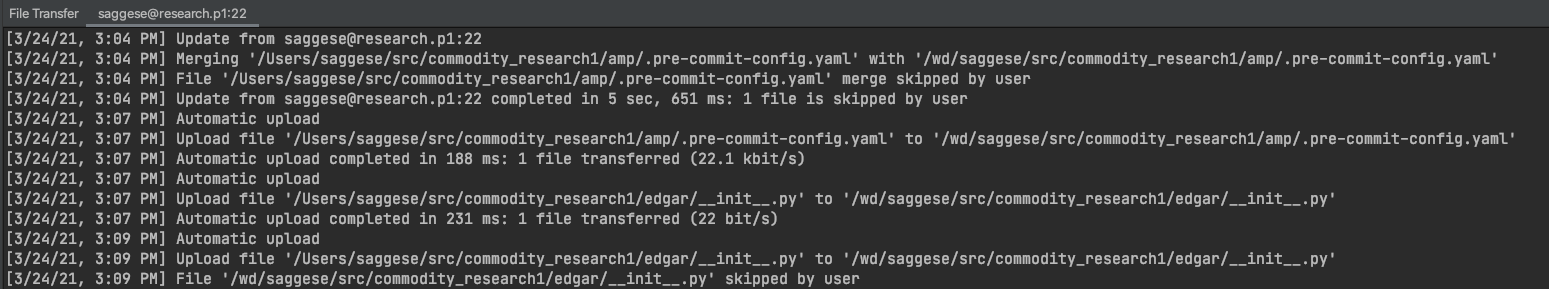
\includegraphics[width=6.5in,height=1.875in]{media/image14.png}

\href{https://lucid.app/lucidchart/9ee80100-be76-42d6-ad80-531dcfee277e/edit?page=0_0\&invitationId=inv_5777ae4b-d8f4-41c6-8901-cdfb93d98ca8\#}{\ul{https://lucid.app/lucidchart/9ee80100-be76-42d6-ad80-531dcfee277e/edit?page=0\_0\&invitationId=inv\_5777ae4b-d8f4-41c6-8901-cdfb93d98ca8\#}}

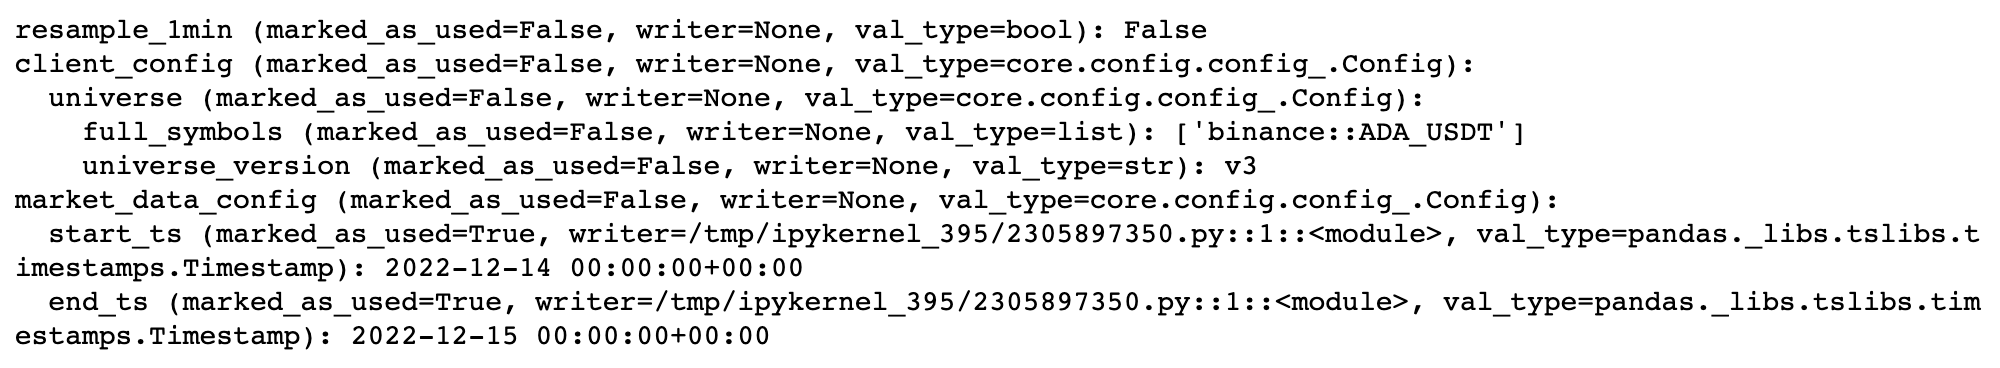
\includegraphics[width=6.5in,height=4.31944in]{media/image13.png}

\textbf{ImClient}

Responsibilities:

Interactions:

Main methods:

\textbf{MarketData}

Responsibilities:

Interactions:

Main methods:

\textbf{Forecaster.} It is a DAG system that forecasts the value of the
target economic quantities (e.g.,

for each asset in the target

Responsibilities:

Interactions:

Main methods:

\textbf{process\_forecasts.} Interface to execute all the predictions in
a Forecast dataframe through TargetPositionAndOrderGenerator.

This is used as an interface to simulate the effect of given forecasts
under different optimization conditions, spread, and restrictions,
without running the Forecaster.

\textbf{TargetPositionAndOrderGenerator}. Execute the forecasts by
generating the optimal target positions according to the desired
criteria and by generating the corresponding orders needed to get the
system from the current to the desired state.

TODO(gp): It also submits the orders so ForecastProcessor?

Responsibilities:

\begin{itemize}
\item
  \begin{quote}
  Retrieve the current holdings from Portfolio
  \end{quote}
\item
  \begin{quote}
  Perform optimization using forecasts and current holdings to compute
  the target position
  \end{quote}
\item
  \begin{quote}
  Generate the orders needed to achieve the target positions
  \end{quote}
\item
  \begin{quote}
  Submit orders to the Broker
  \end{quote}
\end{itemize}

Interactions:

\begin{itemize}
\item
  \begin{quote}
  Forecaster to receive the forecasts of returns for each asset
  \end{quote}
\item
  \begin{quote}
  Portfolio to recover the current holdings
  \end{quote}
\end{itemize}

Main methods:

\begin{itemize}
\item
  \begin{quote}
  compute\_target\_positions\_and\_generate\_orders(): compute the
  target positions and generate the orders needed to reach
  \end{quote}
\item
  \begin{quote}
  \_compute\_target\_holdings\_shares(): call the Optimizer to compute
  the target holdings in shares
  \end{quote}
\end{itemize}

\textbf{Locates}.

\textbf{Restrictions}.

\textbf{Optimizer.}

Responsibilities:

Interactions:

Main methods:

\textbf{Portfolio}. A Portfolio stores information about asset and cash
holdings of a System over time.

Responsibilities:

\begin{itemize}
\item
  \begin{quote}
  hold the holdings in terms of shares of each asset id and cash
  available
  \end{quote}
\end{itemize}

Interactions:

\begin{itemize}
\item
  \begin{quote}
  MarketData to receive current prices to estimate the value of the
  holdings
  \end{quote}
\item
  \begin{quote}
  Accumulate statistics and
  \end{quote}
\end{itemize}

Main methods:

\begin{itemize}
\item
  \begin{quote}
  mark\_to\_market(): estimate the value of the current holdings using
  the current market prices
  \end{quote}
\item
  \begin{quote}
  ...
  \end{quote}
\end{itemize}

\textbf{DataFramePortfolio}: an implementation of a Portfolio backed by
a DataFrame. This is used to simulate a system on an order-by-order
basis. This should be equivalent to using a DatabasePortfolio but
without the complexity of querying a DB.

\textbf{DatabasePortfolio}: an implementation of a Portfolio backed by
an SQL Database to simulate systems where the Portfolio state is held in
a database. This allows to simulate a system on an order-by-order basis.

\textbf{Broker.} A Broker is an object to place orders to the market and
to receive fills, adapting Order and Fill objects to the corresponding
market-specific objects. In practice Broker adapts the internal
representation of Order and Fills to the ones that are specific to the
target market.

Responsibilities:

\begin{itemize}
\item
  \begin{quote}
  Submit orders to MarketOms
  \end{quote}
\end{itemize}

\begin{itemize}
\item
  \begin{quote}
  Wait to ensure that orders were properly accepted by MarketOms
  \end{quote}
\item
  \begin{quote}
  Execute complex orders (e.g., TWAP, VWAP, pegged orders) interacting
  with the target market
  \end{quote}
\item
  \begin{quote}
  Receive fill information from the target market
  \end{quote}
\end{itemize}

Interactions:

\begin{itemize}
\item
  \begin{quote}
  MarketData to receive prices and other information necessary to
  execute orders
  \end{quote}
\end{itemize}

\begin{itemize}
\item
  \begin{quote}
  MarketOms to place orders and receive fills
  \end{quote}
\end{itemize}

Main methods:

\begin{itemize}
\item
  \begin{quote}
  submit\_orders()
  \end{quote}
\item
  \begin{quote}
  get\_fills()
  \end{quote}
\end{itemize}

\textbf{MarketOms}. MarketOms is the interface that allows to place
orders and receive back fills to the specific target market. This is
provided as-is and it\textquotesingle s not under control of the user or
of the protocol

\begin{itemize}
\item
  \begin{quote}
  E.g., a specific exchange API interface
  \end{quote}
\end{itemize}

\textbf{OrderProcessor}

\begin{itemize}
\item
  \begin{quote}
  TODO(gp): Maybe MockedMarketOms since that\textquotesingle s the
  actual function?
  \end{quote}
\end{itemize}

\textbf{OmsDb}

\textbf{\#\# TO REORG}

\# Invariants and conventions

- In this doc we use the new names for concepts and use "aka" to refer
to the

old name, if needed

- We refer to:

- The as-of-date for a query as `as\_of\_timestamp`

- The actual time from `get\_wall\_clock\_time()` as
`wall\_clock\_timestamp`

- Objects need to use `get\_wall\_clock\_time()` to get the "actual"
time

- We don\textquotesingle t want to pass `wall\_clock\_timestamp` because
this is dangerous

- It is difficult to enforce that there is no future peeking when one
object

tells another what time it is, since there is no way for the second
object

to double check that the wall clock time is accurate

- We pass `wall\_clock\_timestamp` only when one "action" happens
atomically but

it is split in multiple functions that need to all share this
information.

This approach should be the exception to the rule of calling

`get\_wall\_clock\_time()`

- It\textquotesingle s ok to ask for a view of the world as of
`as\_of\_timestamp`, but then the

queried object needs to check that there is no future peeking by using

`get\_wall\_clock\_time()`

- Objects might need to get `event\_loop`

- TODO(gp): Clean it up so that we pass event loop all the times and
event

loop has a reference to the global `get\_wall\_clock\_time()`

- The Optimizer only thinks in terms of dollar

\# Implementation

\#\# process\_forecasts()

- Aka `place\_trades()`

- Act on the forecasts by:

- Get the state of portfolio (by getting fills from previous clock)

- Updating the portfolio holdings

- Computing the optimal positions

- Submitting the corresponding orders

- `optimize\_positions()`

- Aka `optimize\_and\_update()`

- Calls the Optimizer

- `compute\_target\_positions()`

- Aka `compute\_trades()`

- `submit\_orders()`

- Call `Broker`

- `get\_fills()`

- Call `Broker`

- For IS it is different

- `update\_portfolio()`

- Call `Portfolio`

- For IS it is different

- It should not use any concrete implementation but only `Abstract*`

\#\# Portfolio

- `get\_holdings()`

- Abstract because IS, Mocked, Simulated have a different
implementations

- `mark\_to\_market()`

- Not abstract

- -\textgreater{} `get\_holdings()`, `PriceInterface`

- `update\_state()`

- Abstract

- Use abstract but make it NotImplemented (we will get some static
checks and

some other dynamic checks)

- We are trying not to mix static typing and duck typing

- CASH\_ID, `\_compute\_statistics()` goes in `Portolio`

\#\# Broker

- `submit\_orders()`

- `get\_fills()`

\# Simulation

\#\# DataFramePortfolio

- This is what we call `Portfolio`

- In RT we can run `DataFramePortfolio` and `ImplementedPortfolio` in
parallel

to collect real and simulated behavior

- `get\_holdings()`

- Store the holdings in a df

- `update\_state()`

- Update the holdings with fills -\textgreater{}
`SimulatedBroker.get\_fills()`

- To make the simulated system closer to the implemented

\#\# SimulatedBroker

- `submit\_orders()`

- `get\_fills()`

\# Implemented system

\#\# ImplementedPortfolio

- `get\_holdings()`

- Check self-consistency and assumptions

- Check that no order is in flight otherwise we should assert or log an

error

- Query the DB and gets you the answer

- `update\_state()`

- No-op since the portfolio is updated automatically

\#\# ImplementedBroker

- `submit\_orders()`

- Save files in the proper location

- Wait for orders to be accepted

- `get\_fills`

- No-op since the portfolio is updated automatically

\# Mocked system

- Our implementation of the implemented system where we replace DB with
a mock

- The mocked DB should be as similar as possible to the implemented DB

\#\# DatabasePortfolio

- `get\_holdings()`

- Same behavior of `ImplementedPortfolio` but using `OmsDb`

\#\# DatabaseBroker

- `submit\_orders()`

- Same behavior of `ImplementedBroker` but using `OmsDb`

\#\# OmsDb

- `submitted\_orders` table (mocks S3)

- Contain the submitted orders

- `accepted\_orders` table

- `current\_position` table

\#\# OrderProcessor

- Monitor `OmsDb.submitted\_orders`

- Update `OmsDb.accepted\_orders`

- Update `OmsDb.current\_position` using `Fill` and updating the
`Portfolio`

\hypertarget{section}{%
\subsection{}\label{section}}

\hypertarget{section-1}{%
\subsection{}\label{section-1}}

\hypertarget{universal-pricing-machine}{%
\subsection{\#\# Universal pricing
machine}\label{universal-pricing-machine}}

It promotes efficiency of decentralized digital asset markets by using
financial machine learning to automatically price any digital currency
or token.

It distills knowledge from a large variety of data sources (e.g., news,
social sentiment, financial databases, market data) to automatically
estimate any quantity of interest and its uncertainty, including:

\begin{itemize}
\item
  \begin{quote}
  price, trading volume
  \end{quote}
\item
  \begin{quote}
  risk, volatility
  \end{quote}
\item
  \begin{quote}
  probability of specific events
  \end{quote}
\end{itemize}

for digital assets such as: crypto currency, non-fungible tokens (NFT),
smart contract

at different time scales ranging from seconds to days.

\hypertarget{evaluating-models}{%
\subsection{Evaluating models}\label{evaluating-models}}

The same goal can be achieved with different research pipelines (with
different complexity to set-up and / or execution time):

\begin{itemize}
\item
  \begin{quote}
  Run a model -\textgreater{} results\_df -\textgreater{}
  post-processing + comparison
  \end{quote}
\item
  \begin{quote}
  Run models sweeping the params -\textgreater{} multiple results\_df
  -\textgreater{} comparison
  \end{quote}
\item
\end{itemize}

We want to separate how we compute the metrics and how we apply it

I think we did some work with Max about this, but not sure where it is.

We want to compute metrics (hit rate, pnl, SR, drawdown, \$ per bet,
MAE, AUC) as function of:

\begin{itemize}
\item
  \begin{quote}
  assets
  \end{quote}
\item
  \begin{quote}
  day of the week
  \end{quote}
\item
  \begin{quote}
  time of the day (e.g., between 9am and 10am, 10am and 11am)
  \end{quote}
\item
  \begin{quote}
  liquidity (e.g., how much volume was transacted)
  \end{quote}
\item
  \begin{quote}
  spread (...)
  \end{quote}
\item
  \begin{quote}
  \ldots{}
  \end{quote}
\end{itemize}

There is a common idiom (which we will formalize in the Surrentum
standard). In practice the pipeline is:

\textbf{Step 1 (compute results\_df)}

\begin{itemize}
\item
  \begin{quote}
  Run the model and generate the usual output, then you can save /
  retrieve this output or just compute with the model on the flight
  \end{quote}
\end{itemize}

\begin{itemize}
\item
  \begin{quote}
  The input is a multi-index dataframe in the DataFlow standard
  (results\_df), like:
  \end{quote}
\end{itemize}

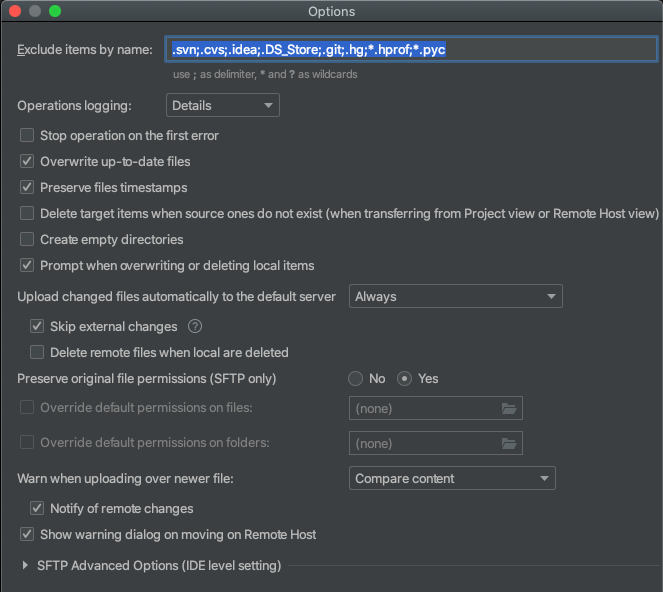
\includegraphics[width=6.5in,height=2.54167in]{media/image9.png}

\textbf{Step 2 (annotate metrics\_df)}

\begin{itemize}
\item
  \begin{quote}
  IMO the best representation is multi-index (timestamp, asset\_id) on
  the rows and columns equal to the features
  \end{quote}

  \begin{itemize}
  \item
    \begin{quote}
    We can call this format "metrics\_df"
    \end{quote}
  \item
    \begin{quote}
    Each row is a prediction of the model
    \end{quote}

    \begin{itemize}
    \item
      \begin{quote}
      Feature1 (price), Feature2 (volume), ...
      \end{quote}
    \end{itemize}
  \item
    \begin{quote}
    (timestamp, asset\_id)
    \end{quote}
  \end{itemize}
\item
  \begin{quote}
  There is a function that annotates each row (timestamp, asset\_id)
  based on certain criteria (e.g., asset\_id, day of the week, a value
  function of a vwap volume)
  \end{quote}

  \begin{itemize}
  \item
    \begin{quote}
    We have a library of function that accept a metrics\_df and then
    decorates it with an extra tag
    \end{quote}
  \item
    \begin{quote}
    E.g., to split the results by asset\_id the function creating the
    tag is something like (timestamp, asset\_id) -\textgreater{} tag =
    asset\_id
    \end{quote}
  \item
    \begin{quote}
    If you want to partition by time of the day you do (timestamp,
    asset\_id) -\textgreater{} tag = timestamp.time()
    \end{quote}
  \item
    \begin{quote}
    \ldots{}
    \end{quote}
  \end{itemize}
\end{itemize}

\textbf{Step 3 (split and compute metrics)}

\begin{itemize}
\item
  \begin{quote}
  There is a function that computes a dict from tag to df (e.g., from
  asset\_id to the corresponding df)
  \end{quote}
\item
  \begin{quote}
  Then we call the function to compute the metric (e.g., hit rate, pnl,
  ...) on each df and build a new dict tag -\textgreater{} transform(df)
  \end{quote}

  \begin{itemize}
  \item
    \begin{quote}
    The transform df accepts various column names to know what is the y,
    y\_hat, ... (this dict is built from the model itself, saying
    what\textquotesingle s the prediction col, the volatility, etc)
    \end{quote}
  \end{itemize}
\end{itemize}

\textbf{Step 4 (aggregate results)}

\begin{itemize}
\item
  \begin{quote}
  Finally we aggregate the results as function of the tag (e.g.,
  asset\_id -\textgreater{} pnl) and plot
  \end{quote}
\item
  \begin{quote}
  The output is a pd.DataFrame (with tag on the rows and metrics on the
  columns)
  \end{quote}
\end{itemize}

\begin{quote}
Metric1

Tag\_value1

\ldots{}
\end{quote}

\begin{itemize}
\item
  \begin{quote}
  E.g., asset\_id -\textgreater{} pnl
  \end{quote}
\end{itemize}

\begin{quote}
asset\_id pnl conf\_int
\end{quote}

\begin{itemize}
\item
  \begin{quote}
  1030\ldots{} \ldots{}
  \end{quote}
\end{itemize}

\hypertarget{building-financial-primitives-with-surrentum-protocol}{%
\section{\# Building financial primitives with Surrentum
Protocol}\label{building-financial-primitives-with-surrentum-protocol}}

\#\# Building a Dark-Pool

\#\# Building algorithmic orders

\#\# Internal matching of orders

\#\# Smart order routing

\#\# Building a synthetic bond

- You like staking because it gives you something to do with your crypto

- You like yield because banks give you 0\% APR and you
don\textquotesingle t have access

to investment opportunities

- Hence all the madness for yield farming

- People creates Ponzi scheme just because there was a huge demand for
yield

but no supply (see the empty box from SBF)

- Meanwhile, our hedge fund needs cash to invest and gives you back the
cash flow

from trading

- But this cash flow is bumpy. One month is good, one month is bad

- You don\textquotesingle t like that

- The typical solution is "pay once a year" so that in average the total
return

is positive, with high watermarks to account from crappy years

- Can we transform our hedge fund bumpy cash flow in something stable,
but worse

in terms of expected return?

- Yes!

- You stake your crypto, we give you 0.5\% / month (6\% a year) in a mix
of cryptos

- We try to give you always ETH and BTC, but sometimes we give you our

Surrentum token

- You can sell or buy Surrentum on the open market as any crypto

- Where does the value of Surrentum come from (i.e., why does it trade
at

more than 0, why is the box not empty)?

- Well, it\textquotesingle s an IOU that we use to make the bumpy cash
flow straight

- As long as the algo makes money in the long run, the Surrentum token
has

value

- Of course we pocket the difference between the 6\% / yr that we pay
users and

the 20\% / yr we made

- Everybody wins

- Financial alchemy achieved!

- This would have been funded instantly few months ago

\hypertarget{related-projects}{%
\section{\# Related projects}\label{related-projects}}

\begin{itemize}
\item
  \begin{quote}
  Numerai
  \end{quote}
\item
  \begin{quote}
  Lean
  \end{quote}
\item
  \begin{quote}
  Quantopian
  \end{quote}
\item
  \begin{quote}
  Crypto-bots (e.g., Pionex)
  \end{quote}
\item
  \begin{quote}
  Amber / FalconX / Talos
  \end{quote}
\item
  \begin{quote}
  HummingbirdBot
  \end{quote}
\item
  \begin{quote}
  https://vega.xyz/
  \end{quote}
\end{itemize}

\hypertarget{refs}{%
\section{\# Refs}\label{refs}}

\href{https://docs.google.com/document/d/1Jp_yPU1FXFF7TdQjLiWzPzTLZmRLJ3KX0dooxArMQeI/edit}{\ul{Surrentum
Protocol - Technical appendix}}

\href{https://docs.google.com/document/d/170IAWtrPUmMGXER-yIEFQ5zaArh2ksRNfvzciF6FLe0/edit\#}{\ul{Surrentum
protocol - Background research}}

\href{https://drive.google.com/drive/u/1/folders/1icv3ifB095AIOMWtgr91v7mfR7Y7KaEl}{\ul{Surrentum
dir}}
